%%%%%%%%%%%%%%%%%%%%%%%%%%%%%%%%%%%%%%%%%
% Stylish Article
% LaTeX Template
% Version 2.2 (2020-10-22)
%
% This template has been downloaded from:
% http://www.LaTeXTemplates.com
%
% Original author:
% Mathias Legrand (legrand.mathias@gmail.com) 
% With extensive modifications by:
% Vel (vel@latextemplates.com)
%
% License:
% CC BY-NC-SA 3.0 (http://creativecommons.org/licenses/by-nc-sa/3.0/)
%
%%%%%%%%%%%%%%%%%%%%%%%%%%%%%%%%%%%%%%%%%

% SNIPPET UTILI %


%----------------------------------------------------------------------------------------
%	PACKAGES AND OTHER DOCUMENT CONFIGURATIONS
%----------------------------------------------------------------------------------------

\documentclass[fleqn,10pt]{SelfArx} % Document font size and equations flushed left

%\usepackage[english]{babel} % Specify a different language here - english by default
\usepackage[italian]{babel} % Specify a different language here - english by default

\usepackage{lipsum} % Required to insert dummy text. To be removed otherwise
\usepackage{attachfile}

%----------------------------------------------------------------------------------------
%	COLUMNS
%----------------------------------------------------------------------------------------

\setlength{\columnsep}{0.55cm} % Distance between the two columns of text
\setlength{\fboxrule}{0.75pt} % Width of the border around the abstract

%----------------------------------------------------------------------------------------
%	COLORS
%----------------------------------------------------------------------------------------

\definecolor{color1}{RGB}{0,0,90} % Color of the article title and sections
\definecolor{color2}{RGB}{0,20,20} % Color of the boxes behind the abstract and headings

%----------------------------------------------------------------------------------------
%	HYPERLINKS
%----------------------------------------------------------------------------------------

\usepackage{hyperref} % Required for hyperlinks

\hypersetup{
	hidelinks,
	colorlinks,
	breaklinks=true,
	urlcolor=color2,
	citecolor=color1,
	linkcolor=color1,
	bookmarksopen=false,
	pdftitle={Title},
	pdfauthor={Author},
}

%----------------------------------------------------------------------------------------
%	ARTICLE INFORMATION
%----------------------------------------------------------------------------------------

\JournalInfo{Programmazione per l'IoT - Laurea Magistrale in Informatica Applicata - DiSPeA - Università degli Studi di Urbino Carlo Bo} % Journal information
\Archive{Data di pubblicazione xx/xx/xxxx - DOI: xxxx/xxxxxxx} % Informazioni che verranno inserite dal Docente in fase di pubblicazione

\PaperTitle{4.0 Gym Prototype} % Article title

\Authors{Luca Cinti\textsuperscript{1}*, Emanuele Lattanzi\textsuperscript{2}} % Il docente Emanuele Lattanzi figura come autore
% al fine di poter gestire la procedura di submission sul repository pubblico (nell'affiliazione viene chiarito il ruolo)
\affiliation{\textsuperscript{1}\textit{Laurea Magistrale in Informatica Applicata, Università degli Studi di Urbino Carlo Bo, Urbino, Italia}} % Author affiliation
\affiliation{\textsuperscript{2}\textit{Docente di Programmazione per l'Internet of Things, Università degli Studi di Urbino Carlo Bo, Urbino, Italia}} % Author affiliation
\affiliation{*\textbf{Corresponding author}: l.cinti@campus.uniurb.it} % Corresponding author

\Keywords{IOT --- Arduino --- ESP32 --- MQTT --- Gym Metrics} % Keywords - if you don't want any simply remove all the text between the curly brackets
\newcommand{\keywordname}{Keywords} % Defines the keywords heading name

%----------------------------------------------------------------------------------------
%	ABSTRACT
%----------------------------------------------------------------------------------------

\Abstract{
	In questo elaborato abbiamo cercato di predisporre un'architettura per la raccolta dei dati
	in una piccola home gym, innanzitutto per verificare la fattibilità nel reperimento di alcune misurazioni, 
	per poi passare all'analisi dei dati raccolti, con l'obiettivo di estrapolare delle metriche significative 
	sia ai fini dell'allenamento, che dello studio delle caratteristiche termiche dell'ambiente.
}

%----------------------------------------------------------------------------------------

\begin{document}

\maketitle % Output the title and abstract box

%\tableofcontents % Output the contents section

\thispagestyle{empty} % Removes page numbering from the first page

%----------------------------------------------------------------------------------------
%	ARTICLE CONTENTS
%----------------------------------------------------------------------------------------

\section*{Introduzione} % The \section*{} command stops section numbering
%\lipsum[1-3] % Dummy text
% and some mathematics $\cos\pi=-1$ and $\alpha$ in the text\footnote{And some mathematics $\cos\pi=-1$ and $\alpha$ in the text.}
%Questa è una citazione al libro di testo~\cite{milenkovic2020internet}.

% \begin{enumerate}[noitemsep] % [noitemsep] removes whitespace between the items for a compact look
% 	\item First item in a list
% 	\item Second item in a list
% 	\item Third item in a list
% \end{enumerate}

% \begin{equation}
% 	\cos^3 \theta =\frac{1}{4}\cos\theta+\frac{3}{4}\cos 3\theta
% 	\label{eq:refname2}
% \end{equation}

% \subsection{Subsection}

% \paragraph{Paragraph} \lipsum[7] % Dummy text
% \paragraph{Paragraph} \lipsum[8] % Dummy text

% \subsection{Subsection}

% \lipsum[9] % Dummy text

% Reference to Figure \ref{fig:results}.

% \begin{figure}[ht]\centering
% 	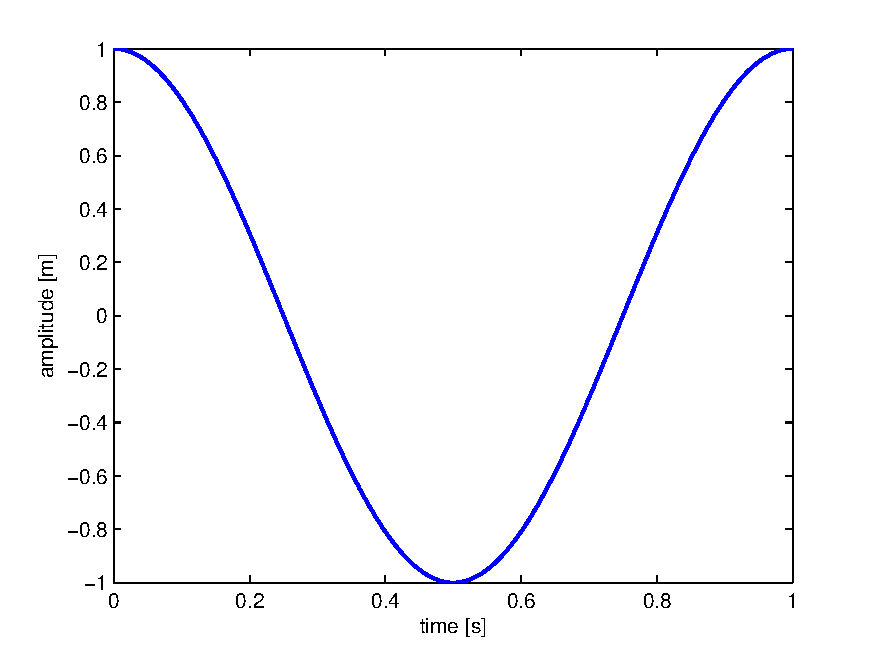
\includegraphics[width=\linewidth]{results}
% 	\caption{In-text Picture}
% 	\label{fig:results}
% \end{figure}

% \begin{description}
% 	\item[Word] Definition
% 	\item[Concept] Explanation
% 	\item[Idea] Text
% \end{description}

L'obiettivo preliminare di questo elaborato era verificare la fattibilità dell'allestimento di un sistema di 
raccolta dati, in una piccola home gym, costruendo l'infrastruttura per far comunicare 
attraverso diversi protocolli una rete di sensori.\\

Tra le più disparate metriche di possibile interesse ai fini dello studio di una palestra, 
sono state scelte due categorie di dati: da un lato i quelli relativi all'ambiente di allenamento, 
dall'altro i dati sull'esecuzione degli esercizi.

Per il progetto corrente sono state dunque prese in analisi le metriche seguenti:

\begin{itemize}[noitemsep] % [noitemsep] removes whitespace between the items for a compact look
	\item temperatura e umidità della stanza, prima durante e dopo l'allenamento
	\item variazione di eCO\textsubscript{2} e eTVOC (equivalent Total Volatile Organic Compounds)
	\item accelerazione del bilanciere durante l'esecuzione di un esercizio campione
\end{itemize}

\section{Descrizione dell'ambiente}

Funzionale alla comprensione di questo elaborato, è la descrizione dell'ambiente in cui è stata allestita 
la palestra: si tratta di una stanza appartenente ad un vecchio immobile disabitato, appositamente 
ristrutturata, le cui misure sono 5.05 x 4.95 metri, per un'altezza di 3.86 metri. \\

L'ambiente presenta una finestra, una porta finestra e un'arcata di ingresso sulla quale sono state applicate 
due tende, fissate con velcro ai lati del muro, come isolante dal resto del locale, in quanto non 
sono presenti sistemi di riscaldamento centralizzato. Possiamo vederne una panoramica nell'immagine che segue 
(Figura 2). \\

Il primo punto di analisi è dunque diretta conseguenza di quanto appena detto: analizzare le performance 
termiche dell'ambiente, per trovare il miglior metodo di riscaldamento durante i mesi invernali.\\
Collegato a questo vi è il secondo punto in analisi: riscaldando un ambiente di circa 96 metri cubici, quanto 
più possibile isolato dal resto del locale, abbiamo ritenuto importante monitorare la qualità dell'aria 
durante l'allenamento.

\subsection{La terza metrica}
Come abbiamo visto in precedenza, come terzo oggetto di studio è stata presa in analisi l'accelerazione del bilanciere 
durante l'esecuzione di un esercizio campione.\\
L'esercizio selezionato è la distensione su panca piana, scelto in quanto ci garantiva il maggior grado di controllo 
sull'esecuzione, essendo uno degli esercizi base di ogni allenamento. Ne possiamo vedere uno schema in Figura 1.\\

La popolarità di tale esercizio ci garantiva inoltre buone potenzialità di espansione di questo studio ad un 
ampio campione di tester, nel caso fossimo riusciti a standardizzare il più possibile il metodo di acquisizione dei dati.

\begin{figure}[htb!]\centering
	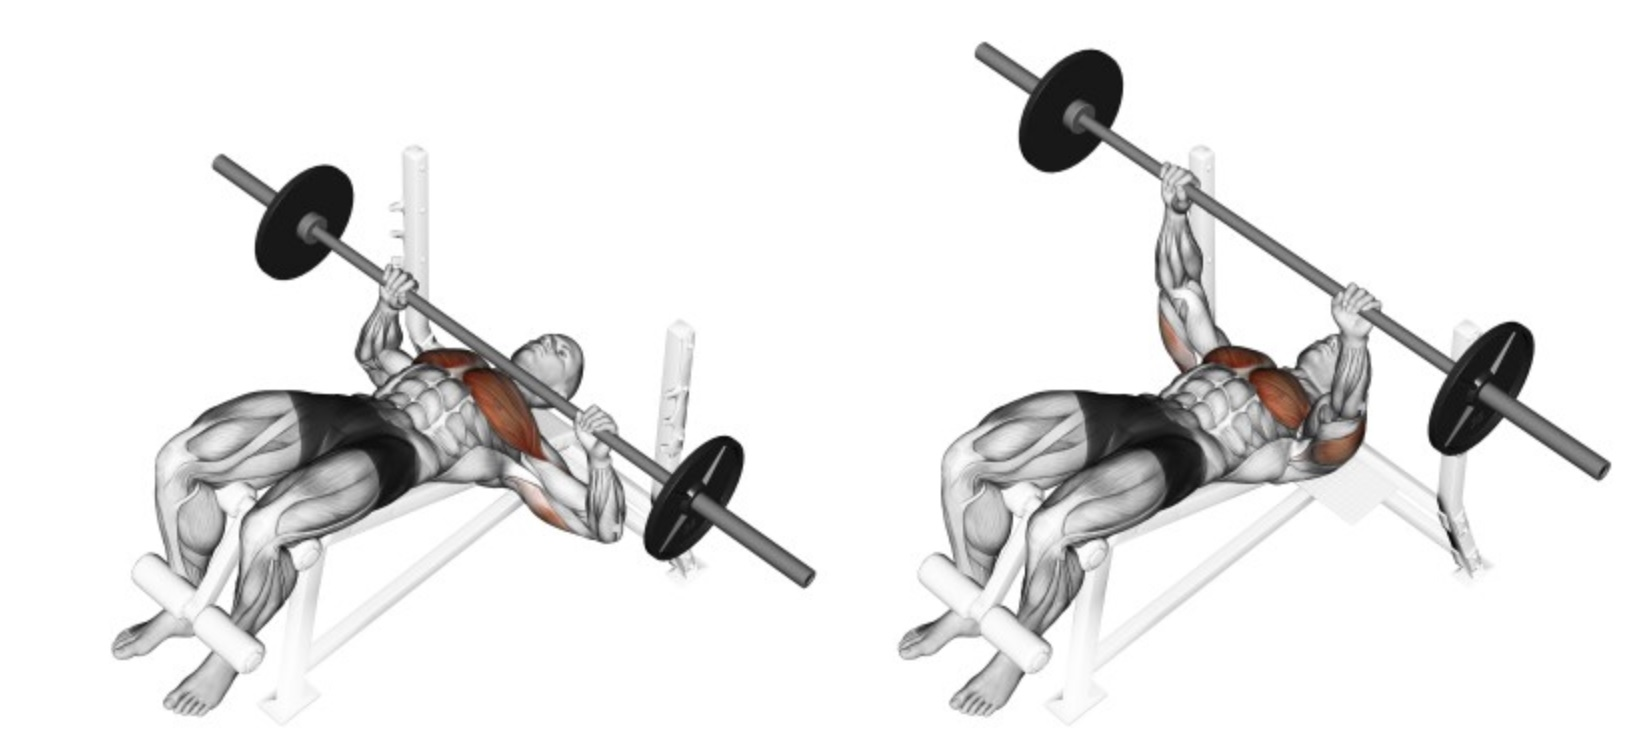
\includegraphics[width=\linewidth]{panca_piana}
	\caption{distensioni su panca piana}
	\label{fig:panca_piana}
\end{figure}

\begin{figure*}[ht]\centering % Using \begin{figure*} makes the figure take up the entire width of the page
	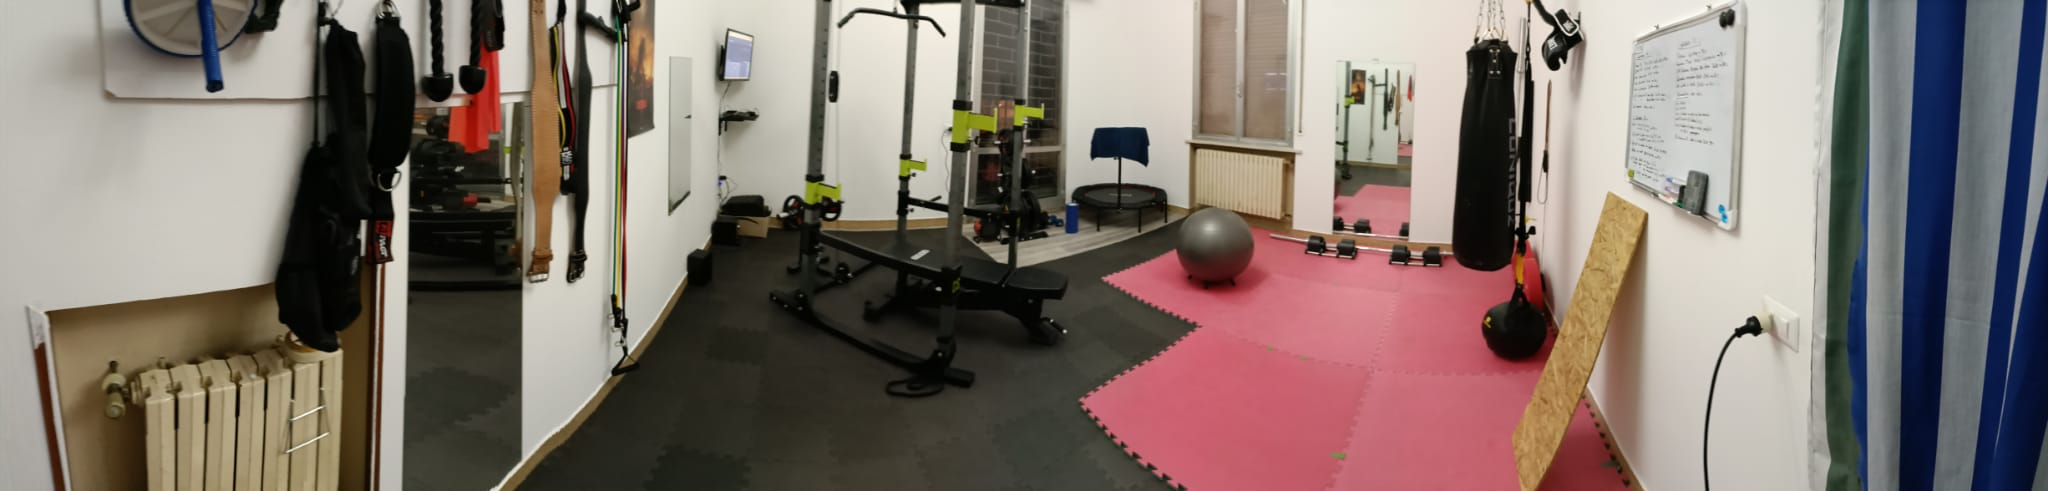
\includegraphics[width=\linewidth]{panoramica_palestra}
	\caption{Visione panoramica dell'ambiente}
	\label{fig:view}
\end{figure*}

%------------------------------------------------

\section{Gli strumenti utilizzati}

In questa sezione porremo l'attenzione sugli strumenti di indagine utilizzati, sulla loro costruzione, 
e sulle scelte di progetto e implementazione adottate.

\subsection{Allestimento dell'infrastruttura}

La prima necessità è stata dunque quella di creare l'infrastruttura attraverso la quale sarebbe avvenuta la 
comunicazione dei dati.\\
A livello di rete e internet sono stati fatti diversi tentativi, prima con due diversi router extender che 
prolungavano una rete casalinga fino al locale della palestra, e poi con un router con scheda SIM 
situato direttamente in loco. La prima soluzione è stata scartata in quanto, ad una distanza in linea d'aria 
dal router di casa di circa cinquanta metri, senza considerare i muri, la connessione era troppo instabile.\\

A questa rete è stato poi collegato un Raspberry Pi 4 che ha fatto sia da broker MQTT (di cui parleremo in seguito), 
che da semplice computer per la raccolta e visualizzazione dei dati, come vediamo in Figura 3.

\begin{figure}[htb!]\centering
	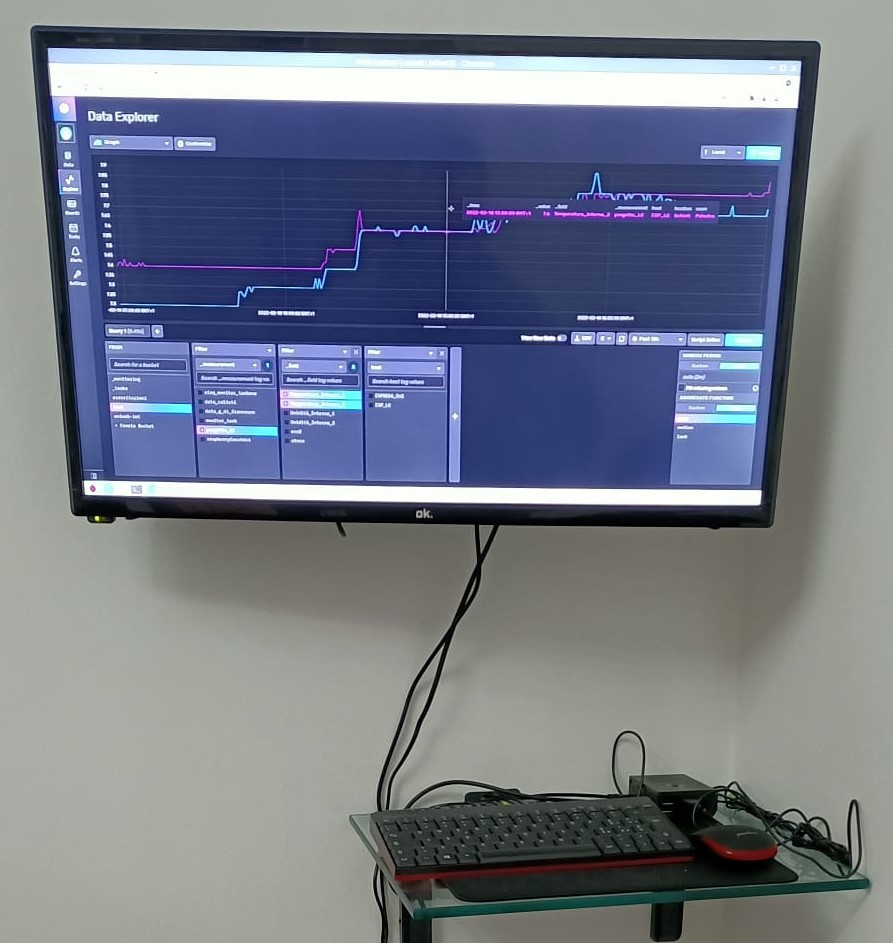
\includegraphics[scale=0.32]{schermo_dati}
	\caption{Raspberry e monitor}
	\label{fig:schermo}
\end{figure}

\subsection{I sensori utilizzati}

Per raccogliere i dati sono stati utilizzati i seguenti sensori:

\begin{itemize}[noitemsep] % [noitemsep] removes whitespace between the items for a compact look
	\item due DHT11 e due DHT22 per temperatura e umidità
	\item un CCS811 per eCO\textsubscript{2} e eTVOC
	\item due GY-521 MPU-6050 per l'accelerazione
\end{itemize}

Si è scelto di collegare gli accelerometri a dei moduli di sviluppo ESP32 mini, potendo così accedere ad 
un'architettura double core, mentre tutti gli altri sensori sono stati collegati a delle normali ESP8266. 
Abbiamo adottato sensori DHT11 e DHT22 per temperatura e umidità, potendo così avere un confronto nella 
precisione dei due: vediamo le differenze tra le loro specifiche nella tabella che segue.

\begin{table}[hbt]
	\caption{Specifiche DHT}
	\centering
	\begin{tabular}{lcc}
		\toprule
			 & \textbf{DHT11} & \textbf{DHT22} \\
		\midrule
		Range umidità & 20-90\% & 0-100\% \\
		Precisione umidità & ±5\% & ±2\% \\
		Range temperatura & 0-50 °C & -40 +80 °C \\
		Precisione temperatura & ±2\% & ±0.5\% \\
		Tempo di lettura & 6-10 s & 2 s \\
		\bottomrule
	\end{tabular}
	\label{tab:label}
\end{table}

Nelle tre immagini che seguono (Figure 4, 5, 6) sono mostrati gli schemi dei circuiti costruiti: 

\begin{figure}[htb!]\centering
	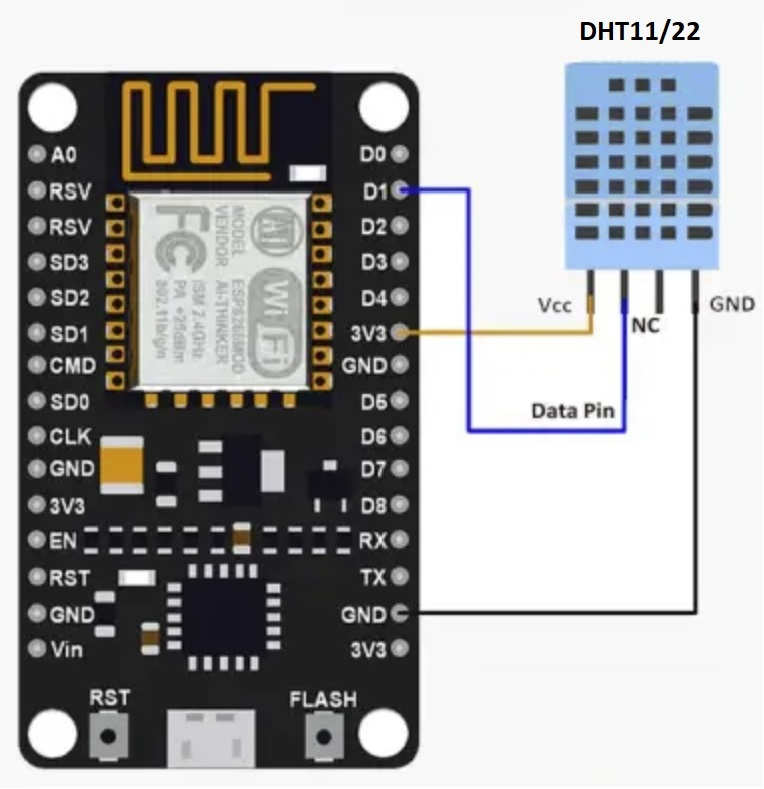
\includegraphics[scale=0.5]{DHT}
	\caption{ESP8266 - DHT11/22}
	\label{fig:DHT11/22}
\end{figure}

\begin{figure}[htb!]\centering
	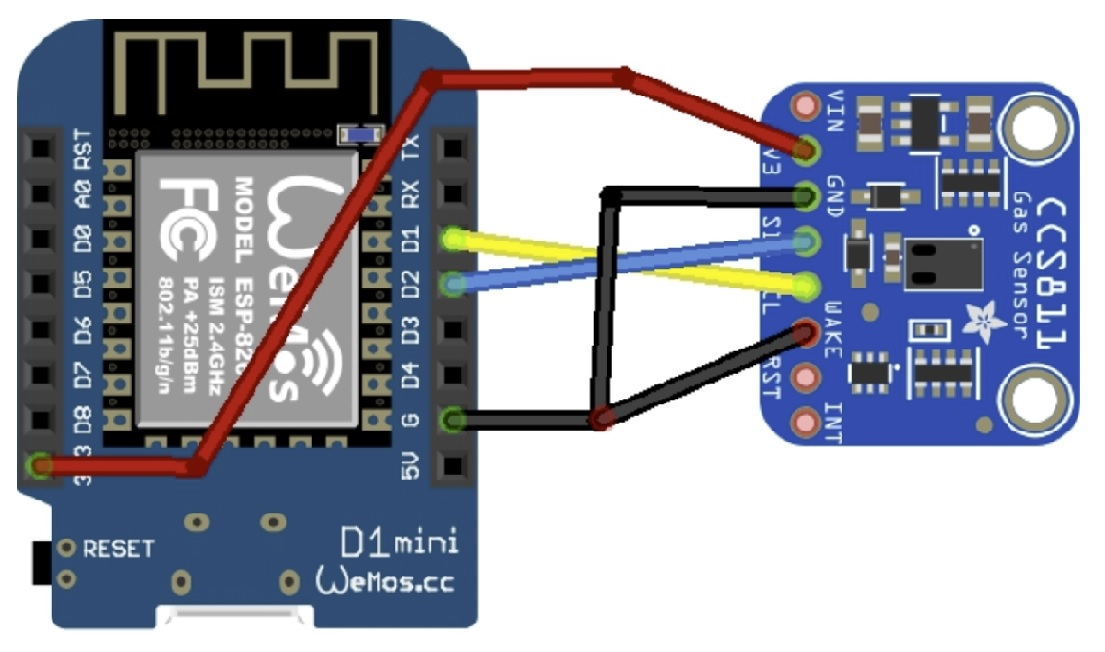
\includegraphics[scale=0.4]{CCS811}
	\caption{ESP8266 - CCS811}
	\label{fig:CCS811}
\end{figure}

\begin{figure}[htb!]\centering
	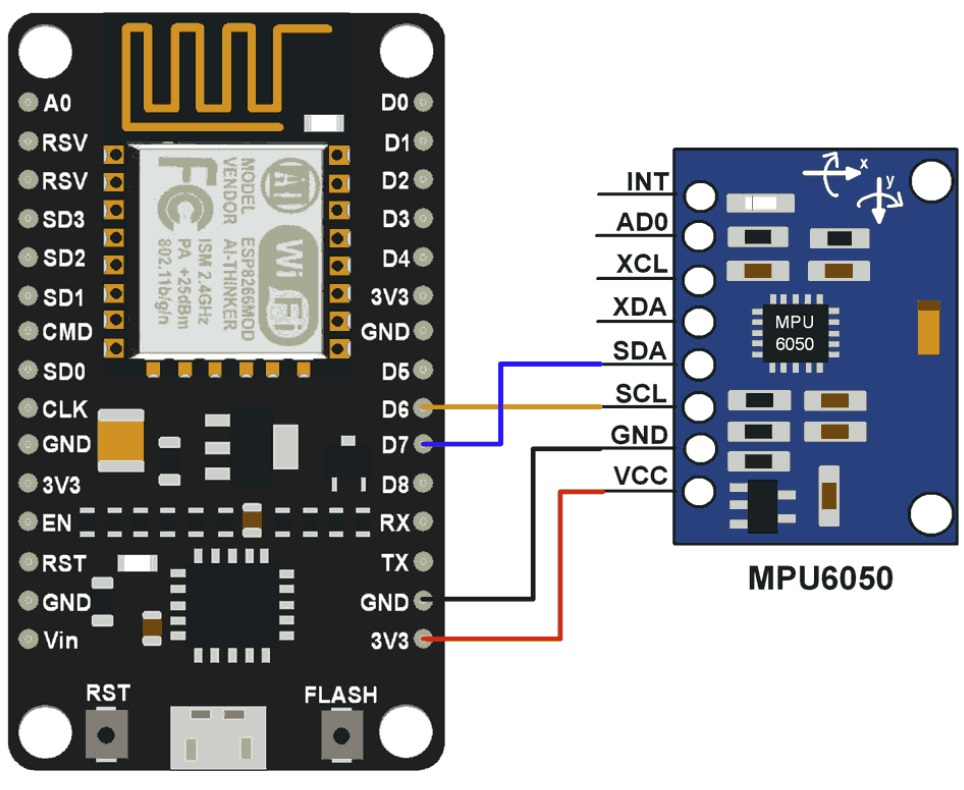
\includegraphics[scale=0.45]{Schema_accelerometro}
	\caption{ESP32 - MPU-6050}
	\label{fig:MPU-6050}
\end{figure}

\subsubsection{I sensori per i dati ambientali e il loro obiettivo}
Tenendo a mente il primo punto di indagine indicato nell'introduzione, ovvero analizzare i dati ambientali, è doveroso 
innanzitutto rispondere al perché abbiamo ritenuto delle metriche tuttosommato banali, 
quali umidità e temperatura, interessanti ai fini dell'elaborato.\\
Come già detto, il locale non presenta sistemi di riscaldamento centralizzato, e, raggiungendo nei mesi invernali 
temperature interne prossime agli zero gradi centigradi, si è scelto di riscaldarlo tramite un generatore di calore a 
GPL con una potenza di 10 KW, posizionato all'ingresso della palestra, ovvero con la parte frontale dentro il locale, 
e lo scarico fuori (si faccia riferimento alla Figura 7).\\

\begin{figure}[htb!]\centering
	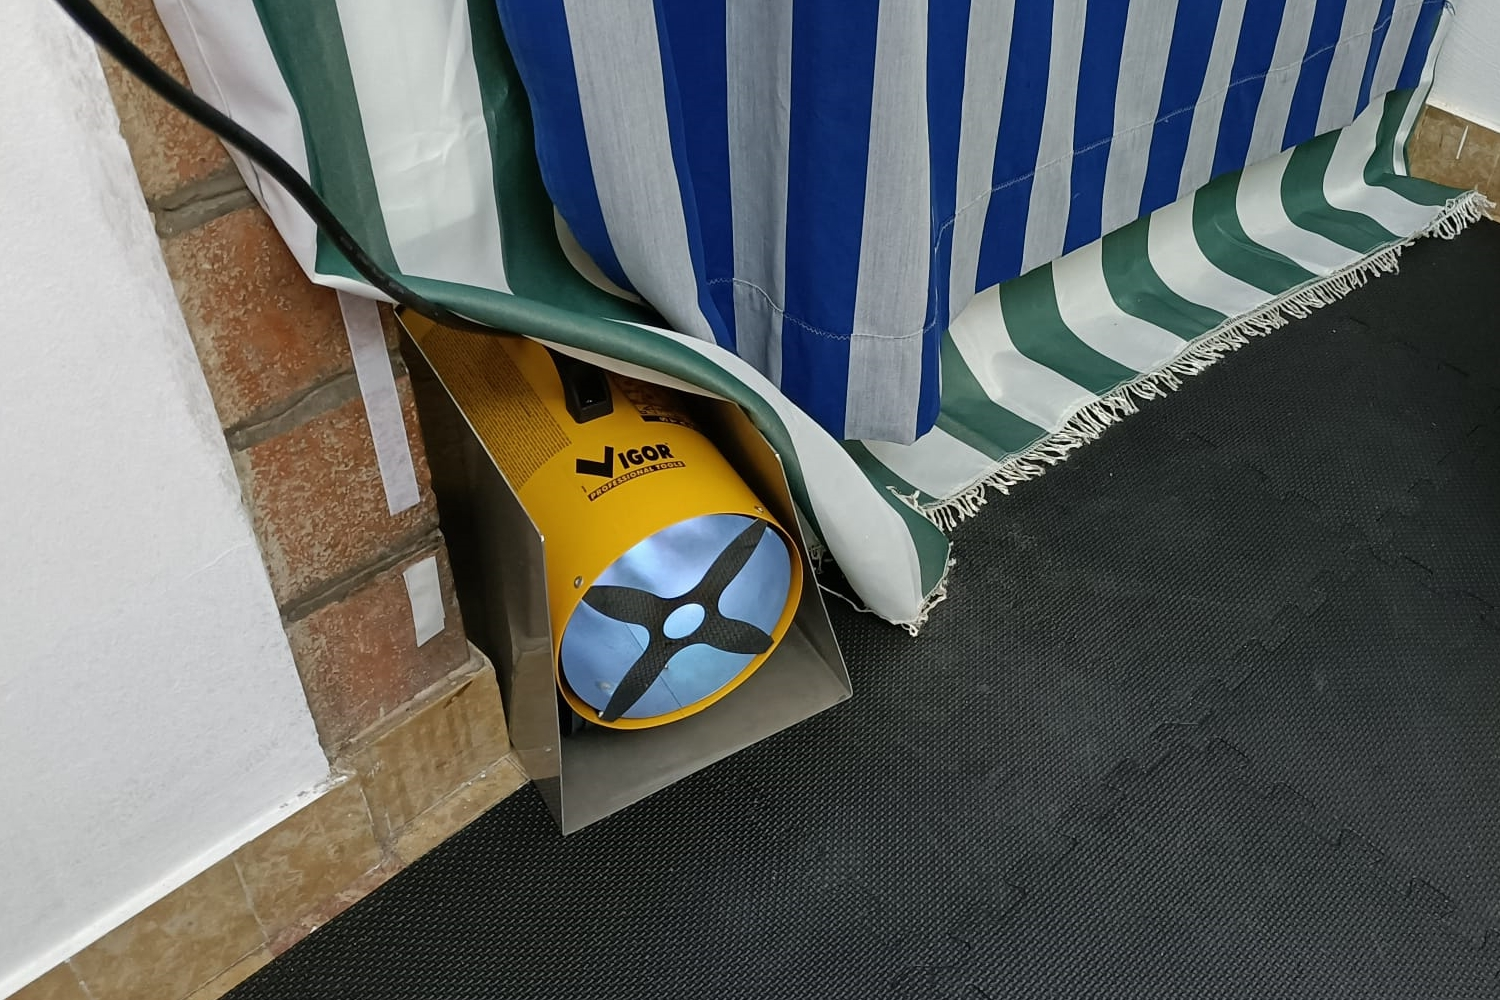
\includegraphics[width=\linewidth]{termoventilatore}
	\caption{Termoventilatore GPL}
	\label{fig:termoventilatore}
\end{figure}

Tuttavia questo presentava altri problemi, sia a livello di sicurezza, trattandosi pur sempre di una combustione 
in un ambiente chiuso, per quanto la zona di scarico fosse sufficientemente grande e areata, che a livello pratico:
il generatore di calore utilizzato è in grado di portare l'ambiente ad una temperatura confortevole in tempi 
contenuti, dell'ordine di dieci/quindici minuti (chiaramente in base alla temperatura di partenza), è dunque 
necessario spegnerlo per non surriscaldare l'ambiente. Questo comporta però un crollo della temperatura pressoché 
immediato. Si è scelto dunque di inserire una stufa da 3 KW il cui compito è quello di mantenere la temperatura costante.\\
Alla luce di quanto detto, assume ancora più importanza la seconda metrica oggetto di studio, ovvero la 
variazione di eCO\textsubscript{2} e eTVOC (equivalent Total Volatile Organic Compounds), come monitor indiretto della 
qualità dell'aria.\\
Importante ricordare a tal proposito che il sensore CCS811 non misura direttamente l'anidride carbonica o i composti organici 
volatili, ma misura la quantità equivalente di impurità nell'aria per ottenere quelle letture del sensore: in altre parole, 
il sensore legge determinati dati di qualità dell'aria, tali dati possono essere dati dalla presenza di CO\textsubscript{2}, 
o da composti organici equivalenti capaci di dare quel tipo di letture. È una sottigliezza ininfluente ai fini dell'elaborato, 
ma per dovere di chiarezza ne abbiamo ritenuto necessaria la precisazione.\\

Data questa premessa passiamo ora a descrivere le relative scelte di progetto.\\
Fare uno studio accurato delle performance termiche di un ambiente richiede una grande quantità di dati, sia a livello 
di caratteristiche ingegneristiche e architettoniche dell'ambiente, che dei materiali di costruzione, informazioni 
alle quali non avevamo completo accesso. Potevamo tuttavia estrapolarle e farne una buona stima, sia attraverso 
l'analisi in loco di periti tecnici, che dai dati restituiti dai sensori.\\

Il dato che si è scelto di ricercare è la dispersione del calore dall'ambiente, che costituisce un buon aggregato e 
indice delle performance termiche della stanza.\\
Per ottenere tale informazione si è scelto di utilizzare i quattro sensori DHT come segue: due sono stati 
posizionati a due angoli della stanza, per ottenere la temperatura media interna, uno fuori dall'edificio per la 
temperatura esterna, e uno appena fuori dall'ingresso della palestra, comunque in un ambiente interno, ma non riscaldato.
\\
Le due postazioni di rilevamento di temperatura e umidità esterne alla stanza, non avendo accesso a prese elettriche, 
sono state implementate con batteria e un con meccanismo di \textit{deep sleep} per il risparmio energetico. 
I relativi circuiti sono stati quindi dotati di collegamenti per una batteria da 650 mA e di un jumper per consentire la 
programmazione del modulo.

\subsubsection{Gli accelerometri e il loro obiettivo}

Un discorso a parte va fatto per gli accelerometri, che per noi costituivano l'argomento di maggiore interesse 
di questo studio.\\
Innanzitutto è necessario chiarire l'obiettivo dell'analisi, ovvero cercare di registrare 
se, nell'esecuzione di un qualsiasi esercizio che coinvolga il sollevamento di un bilanciere, si rilevano delle 
imperfezioni, da cogliere attraverso le differenze nelle accelerazioni agli estremi dell'attrezzo: se un accelerometro 
posto a un estremo del bilanciere, avesse riscontrato accelerazioni diverse da quelle registrate 
all'estremo opposto, sarebbe stato possibile individuare degli errori nell'esecuzione dell'esercizio, 
dandoci così un feedback sulla qualità dello stesso, ed eventuali indicazioni per migliorarlo.\\

Con questo obiettivo in mente abbiamo ritenuto imprescindibile che entrambi i moduli fossero alimentati a batteria, 
per evitare perturbazioni nelle misurazioni dovute ad eventuali interferenze dei fili di alimentazione. Questo ha però 
aumentato la difficoltà nella costruzione del "sistema accelerometro", che includendo ora anche una batteria, 
diventava più ingombrante e difficilmente stabilizzabile sul bilanciere.\\

La soluzione che abbiamo adottato è stata quella di progettare delle scatole di plastica, appositamente 
disegnate in base alle misure del modulo ESP32 col sensore e la batteria, stampate in 3D. Per minimizzare le vibrazioni 
e i movimenti interni alla scatola, sono stati poi inseriti degli spessori in gommapiuma e dei tappi in plastica, 
aumentando così la stabilità del sistema. Ogni scatola presenta inoltre un foro per accedere alla porta USB dell'ESP32 
per le future programmazioni del modulo.\\
Ne possiamo vedere il risultato nella Figura 8.

\begin{figure}[htb!]\centering
	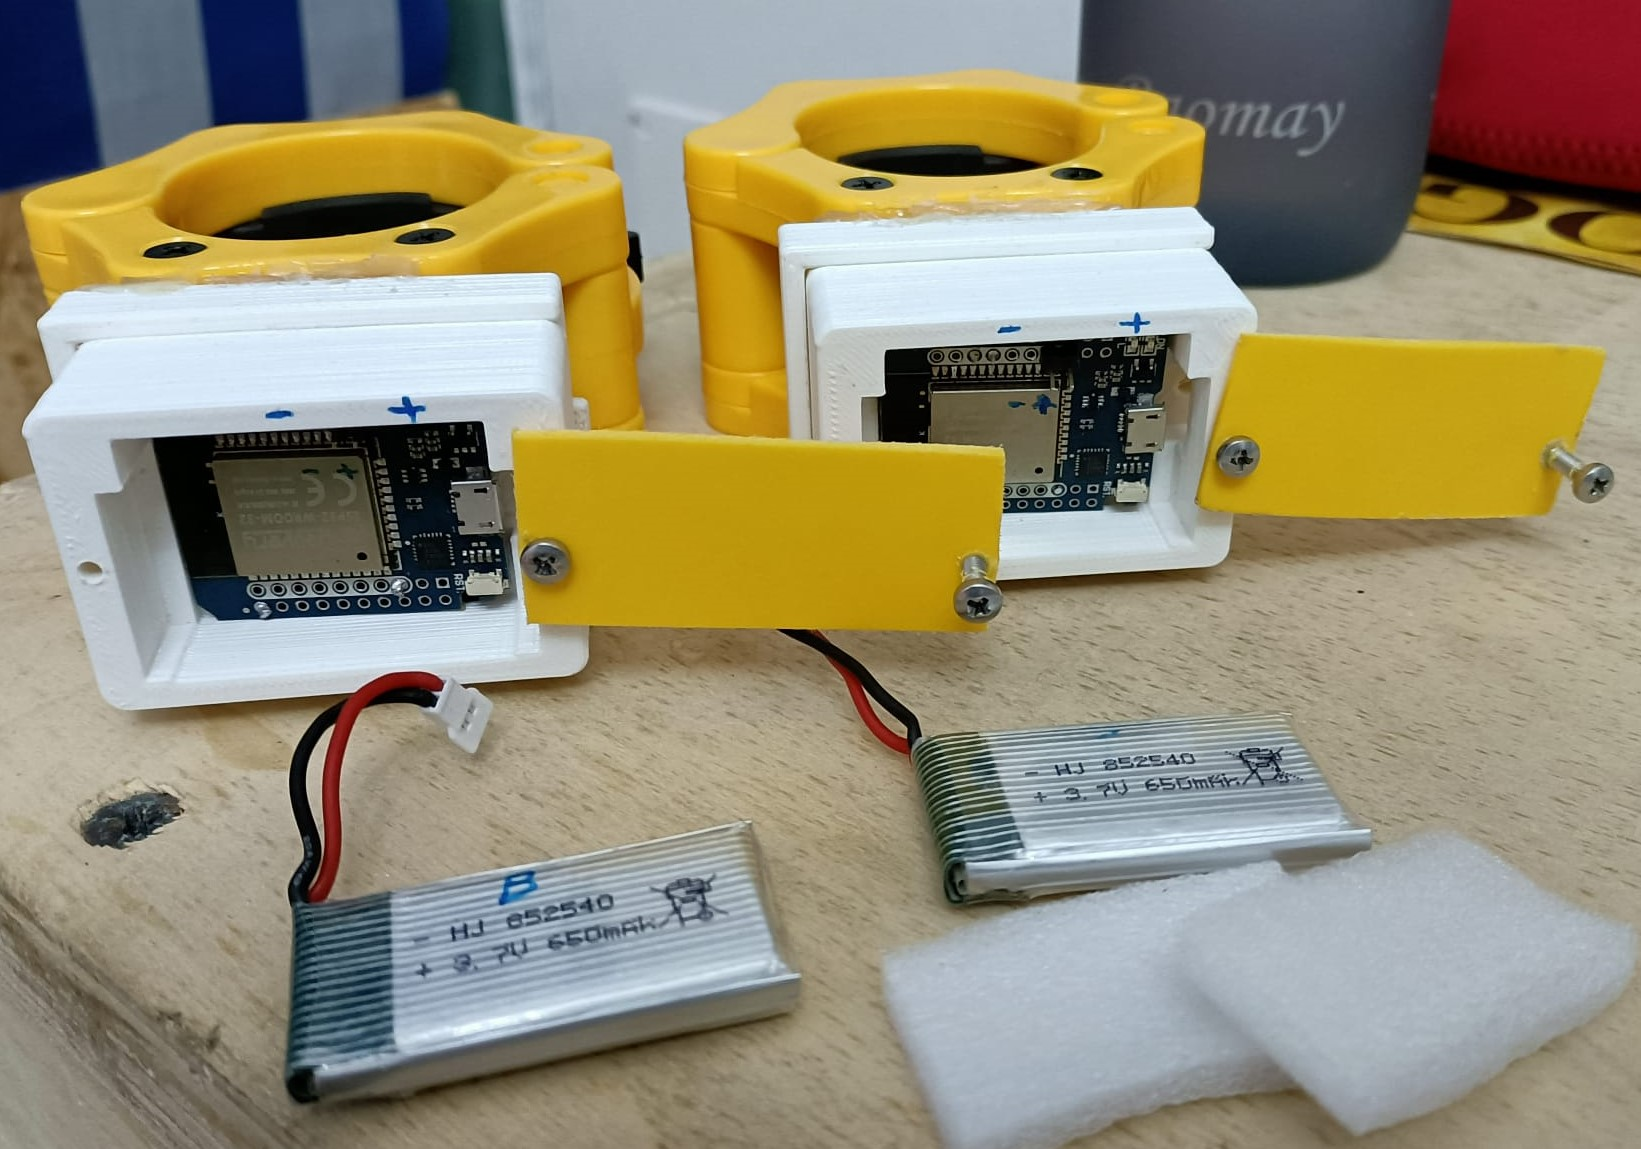
\includegraphics[width=\linewidth]{scatole_accelerometri}
	\caption{Scatola con accelerometro}
	\label{fig:modulo accelerometro}
\end{figure}

Queste scatole sono state poi fissate agli anelli di bloccaggio dei dischi al bilanciere, come vediamo in Figura 9.

\begin{figure}[htb!]\centering
	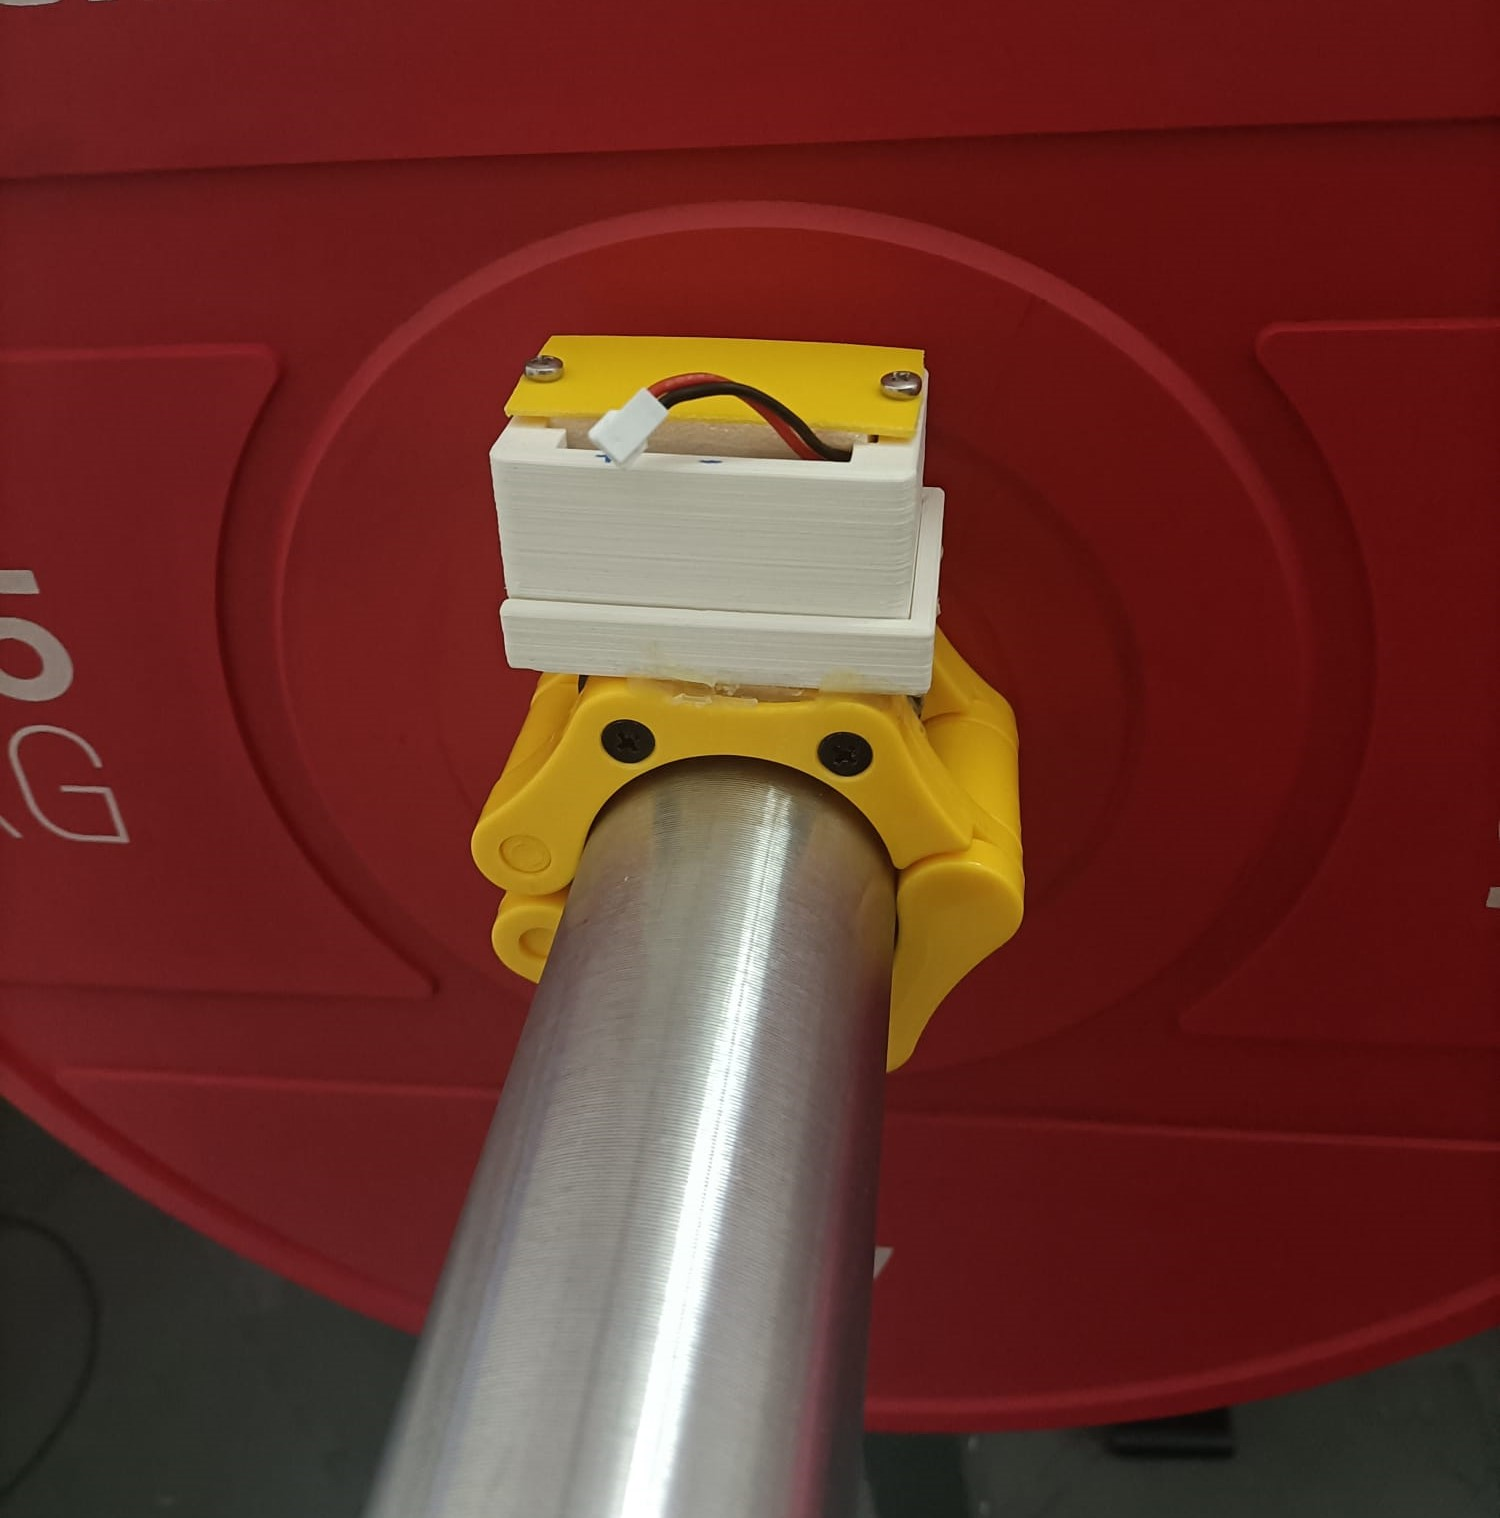
\includegraphics[scale=0.15]{disco_bilanciere}
	\caption{Anello di bloccaggio dischi su bilanciere}
	\label{fig:anello di bloccaggio}
\end{figure}

Aggiungiamo inoltre che i bilancieri utilizzati per questi test sono bilancieri standard olimpici, di cui riportiamo 
le misure nell'immagine che segue (Figura 10), che hanno, e questo vedremo in seguito che risulterà critico, 
la caratteristica di avere la zona di fissaggio dei pesi capace di ruotare attorno all'asse del bilanciere. \\
Tale accorgimento tecnico si utilizza per minimizzare la rotazione, e le conseguenti accelerazione e variazione 
di momento angolare del sistema, in fase di movimento del carico: un'improvvisa rotazione del bilanciere attorno 
al suo asse orizzontale non comporta così la rotazione dei pesi (o comunque la riduce significativamente), 
che causerebbe maggiore instabilità nell'esercizio.

\begin{figure}[htb!]\centering
	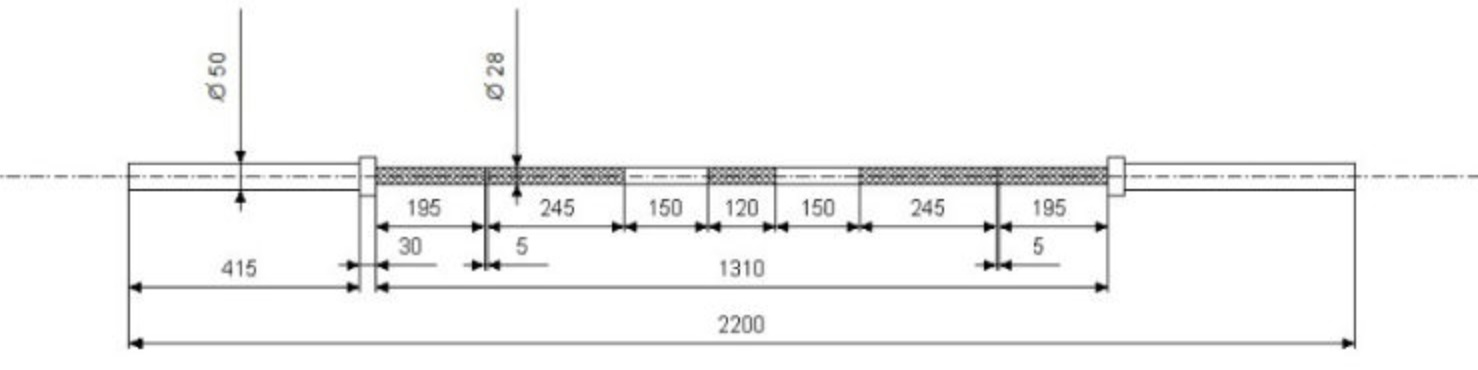
\includegraphics[width=\linewidth]{bilanciere}
	\caption{Misure bilanciere olimpico}
	\label{fig:bilanciere}
\end{figure}

Prima di passare alla raccolta e analisi dei dati ci è doveroso aggiungere che tutti i microcontrollori sono stati 
programmati tramite Arduino. Eventuali particolarità o dettagli specifici di implementazione saranno affrontati in fase 
di analisi dei dati. \\
Tutto il codice è comunque consultabile nella repository GitHub indicata in bibliografia.

\section{Raccolta dati}

I dati sono stati raccolti su un server remoto sul quale è stato installato \textit{influxdb}, un database open source 
per serie temporali, particolarmente adatto ad applicazioni IOT.\\

Dei sette sensori di cui si è discusso, cinque comunicavano tramite il modulo WiFi del microcontrollore collegandosi 
direttamente al server remoto.\\

\begin{figure}[htb!]\centering
	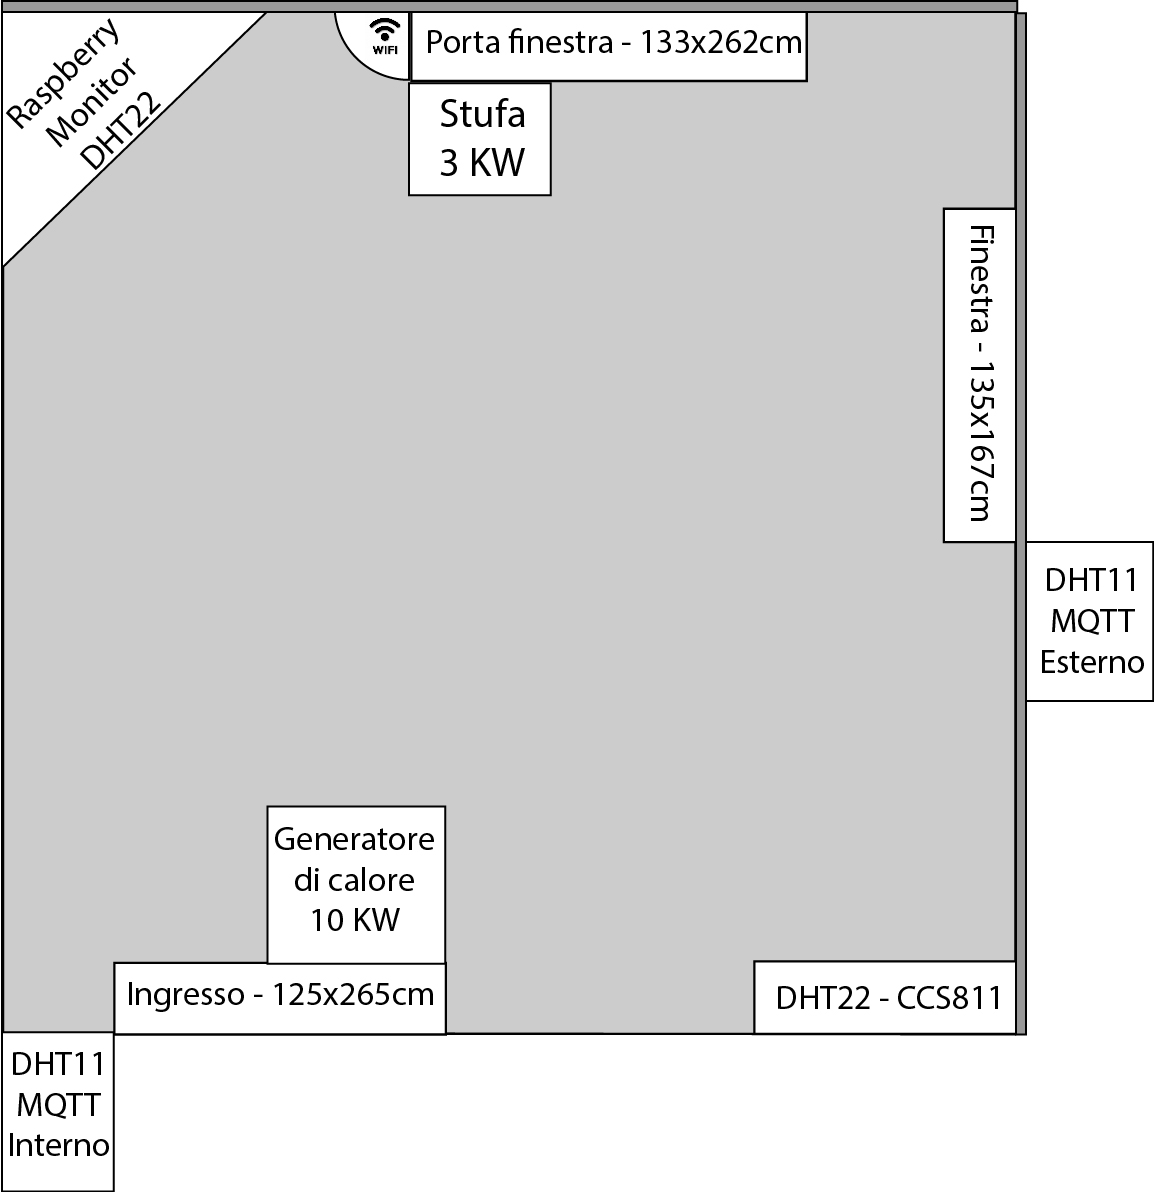
\includegraphics[width=\linewidth]{pianta_palestra}
	\caption{Pianta della palestra. Non in scala}
	\label{fig:pianta palestra}
\end{figure}

Per i due moduli con DHT11 posizionati fuori dalla palestra, quello interno al locale, e quello esterno all'edificio 
(per maggior chiarezza si faccia riferimento alla pianta del locale in Figura 11) si è optato per una soluzione 
differente: essendo alimentati a batteria, abbiamo scelto di utilizzare due tecnologie particolarmente adatte al 
risparmio energetico. Come protocollo di comunicazione si è scelto MQTT (Message Queuing Telemetry Transport), 
particolarmente meno energivoro del classico WiFi, con il Raspberry Pi 4, come precedentemente detto, che funge 
da broker, e i due sensori da client. \\
Per l'invio dei dati su influxdb è stato poi appositamente configurato su Raspberry un \textit{plugin telegraf}.\\
La seconda tecnologia per il risparmio energetico è più che altro un accorgimento a livello implementativo: invece di 
programmare i sensori con la classica modalità, ovvero in loop continuo, si è scelto di adottare il \textit{deep sleep}, 
ovvero al termine di ogni lettura e invio dati, i moduli vengono letteralmente addormentati, lasciando attivo il Real 
Time Clock (RTC), che si occupa di risvegliare il sistema dopo un intervallo di tempo programmabile.\\
Nel nostro caso abbiamo visto che la durata della batteria, con questo accorgimento, è praticamente decupliata, 
passando da circa cinque ore a oltre due giorni.\\
Nell'immagine che segue (Figura 12) vediamo uno dei due sensori in oggetto.

\begin{figure}[htb!]\centering
	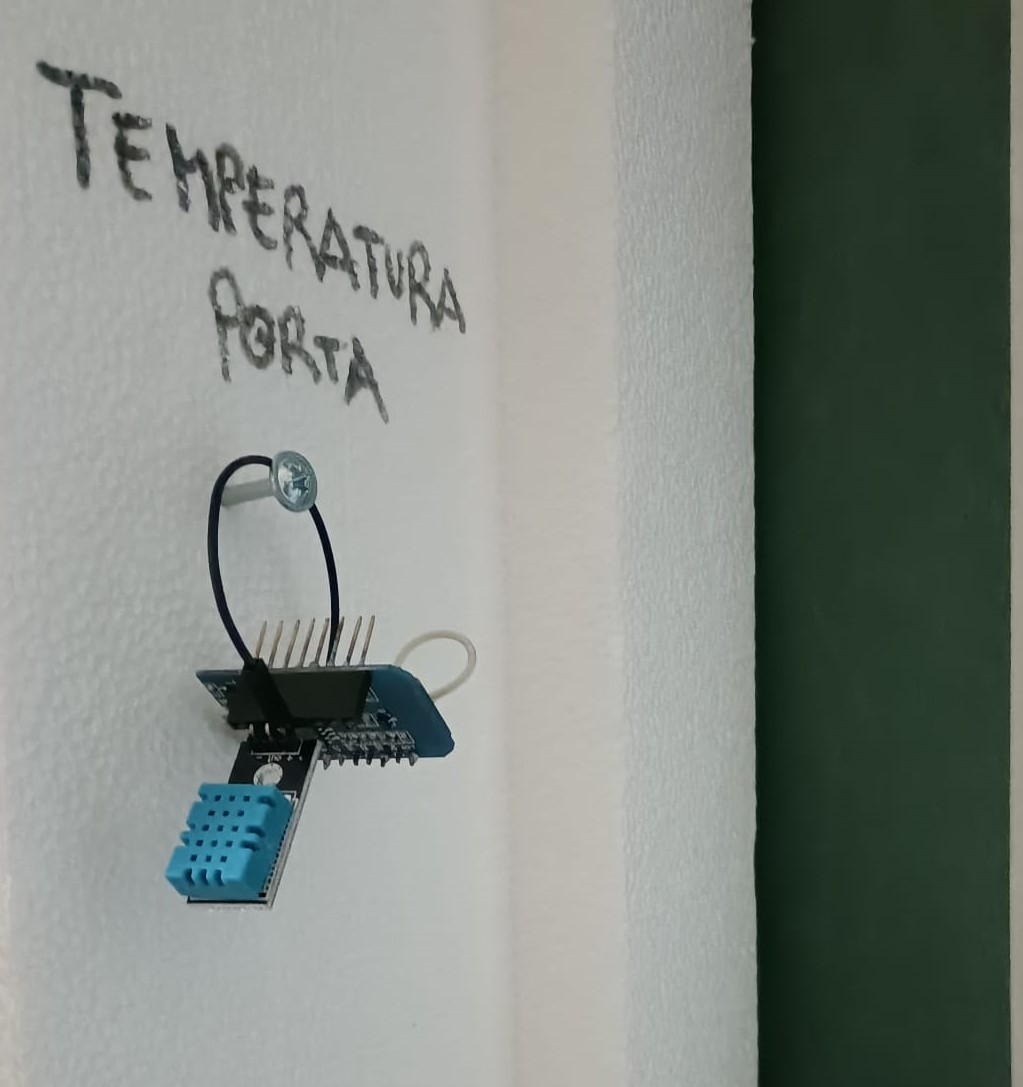
\includegraphics[width=\linewidth]{DHT-MQTT}
	\caption{Sensore DHT11 fuori dall'ingresso della palestra}
	\label{fig:DHT11 MQTT}
\end{figure}

\section{I dati ambientali durante l'allenamento}

Premettiamo che tutti i dati sono disponibili sia in forma aggregata che estensivamente nella repository GitHub indicata 
in bibliografia, oltre ad essere consultabili direttamente sul server influxdb.\\

Passiamo ora vedere i dati raccolti, relativi ad una data campione particolarmente indicativa, in cui è stata utilizzata 
la palestra. Alleghiamo i grafici estratti da influxdb nelle immagini che seguono (Figure 13, 14, 15), e 
condensati nella tabella in Figura 16.\\

\begin{figure}[htb]\centering
	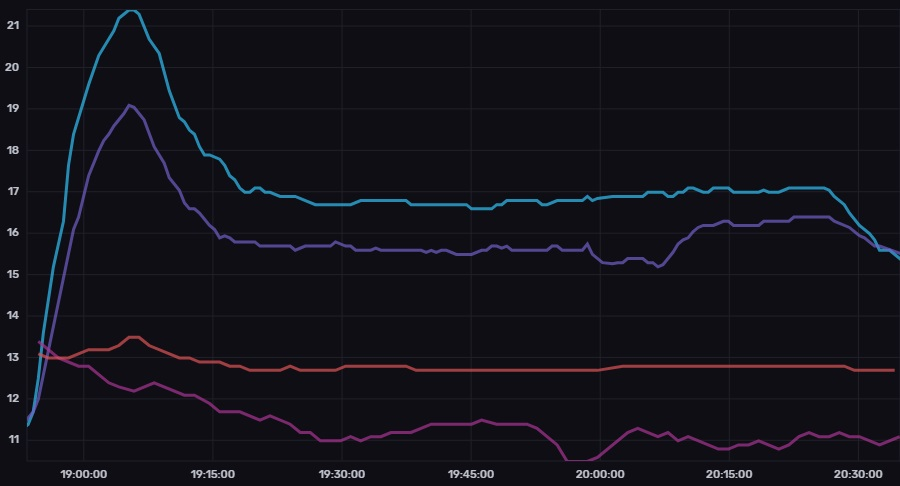
\includegraphics[width=\linewidth]{temperature_2102}
	\caption{Temperatura in gradi Celsius}
	\label{fig:Variazione temperatura}
\end{figure}
\begin{figure}[htb]\centering
	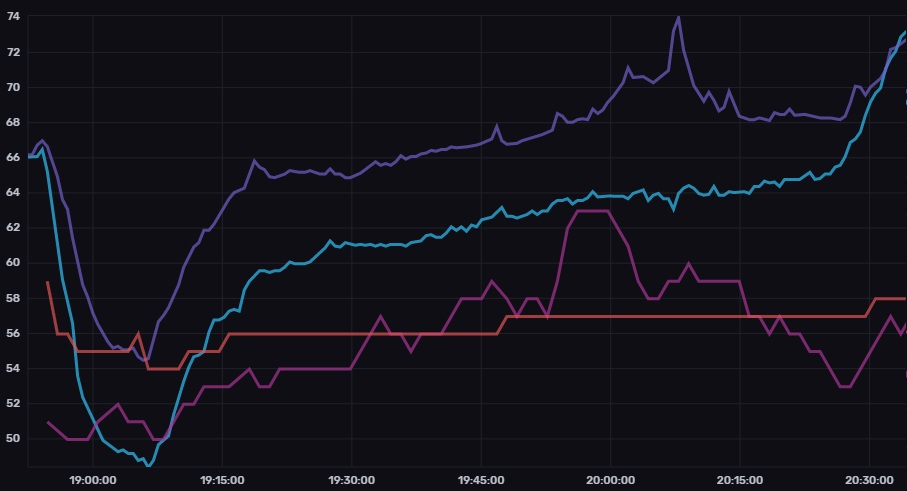
\includegraphics[width=\linewidth]{umidita_2102}
	\caption{Umidità in percentuale}
	\label{fig:Variazione umidità}
\end{figure}
\begin{figure}[htb]\centering
	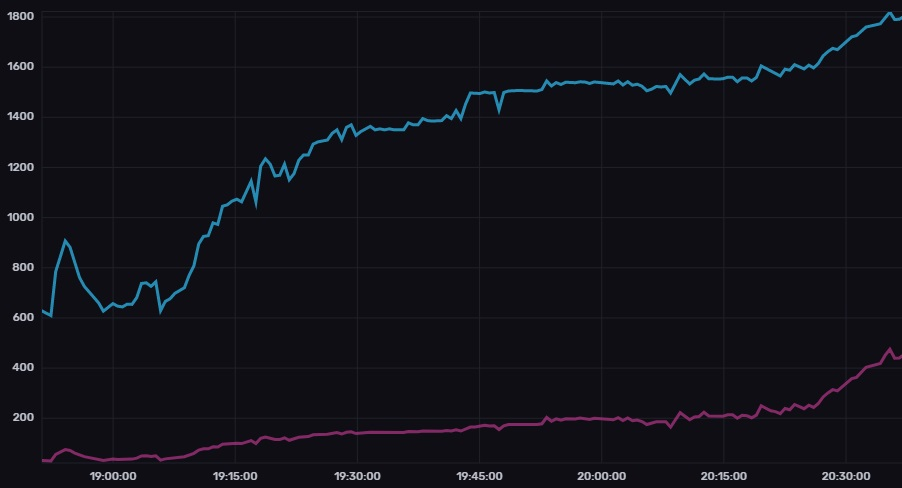
\includegraphics[width=\linewidth]{co2_2102}
	\caption{eCO\textsubscript{2} in ppm e eTVOC in ppb}
	\label{fig:Variazione CO2}
\end{figure}

Le linee azzurre e viola sono relative ai due sensori interni, quella arancio 
al sensore fuori dall'ingresso, quella magenta al sensore esterno.

\begin{figure}[htb]\centering
	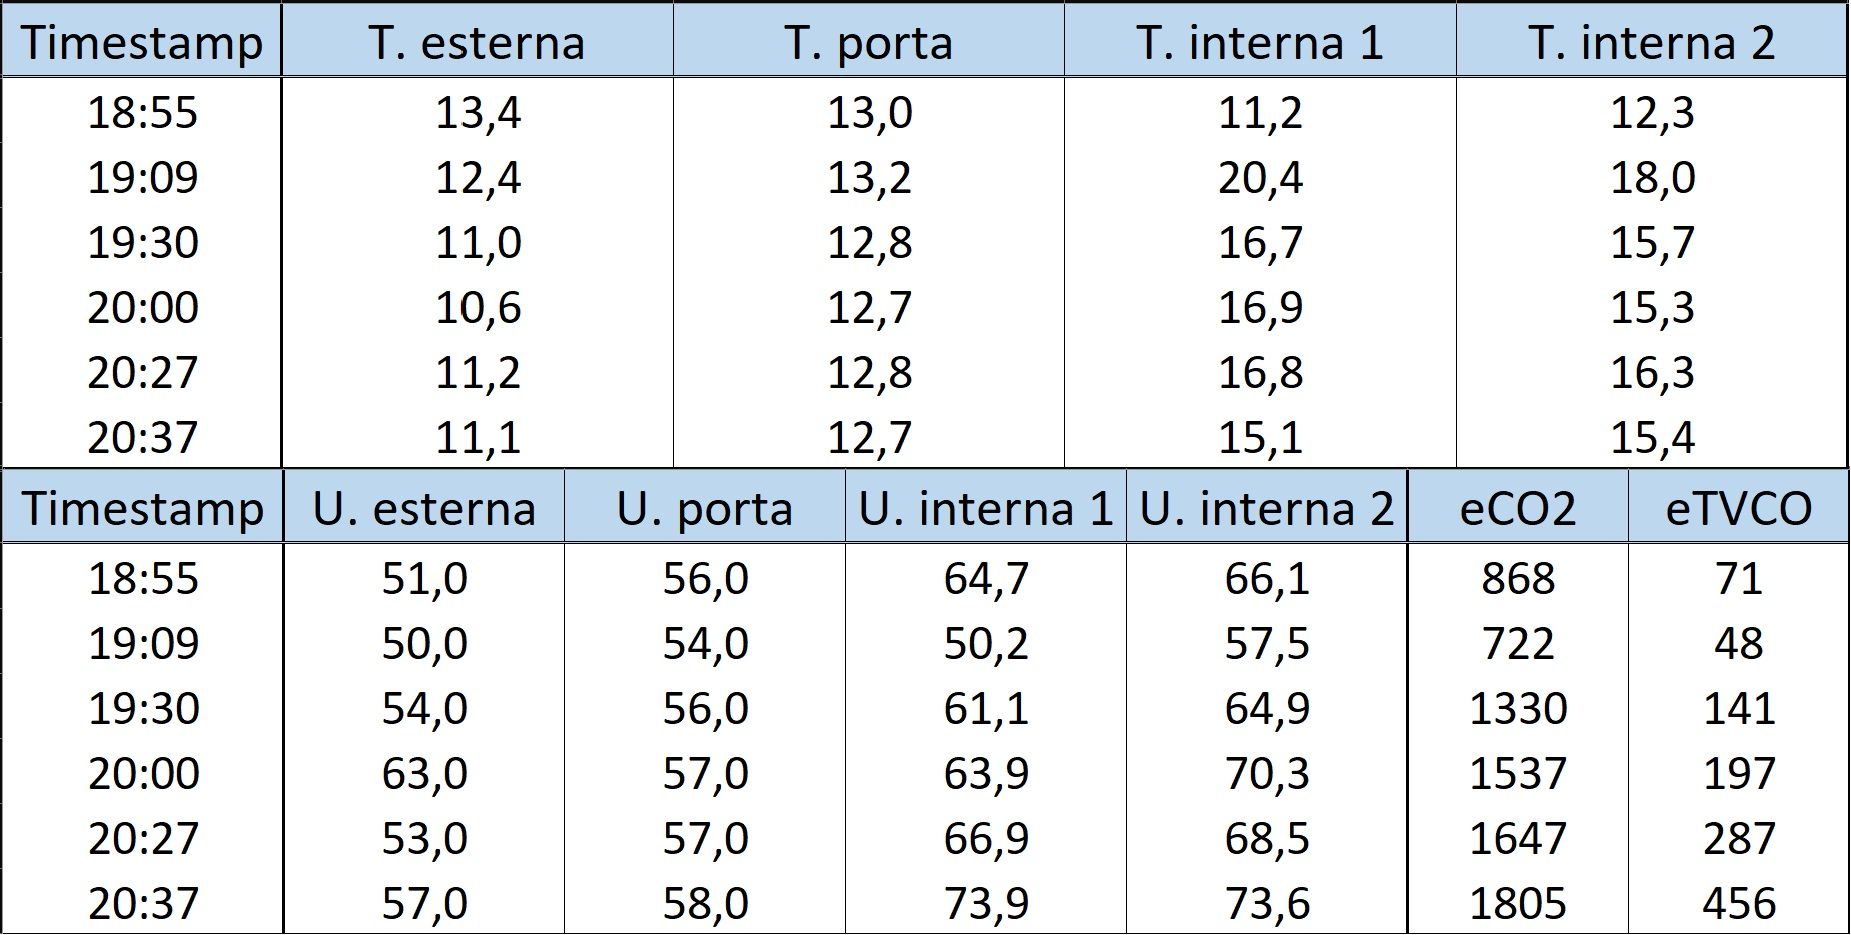
\includegraphics[width=\linewidth]{tabella_dati}
	\captionsetup{width=\linewidth}
	\caption{dati condensati in timestamp significativi}
	\label{fig:tabella dati}
\end{figure}

\subsection{Analisi dei dati ambientali}
Iniziamo questa analisi da una descrizione più approfondita dei grafici precedentemente allegati.\\
Come possiamo vedere in tabella, sono stati indicati dei timestamp significativi: 

\begin{itemize}[noitemsep] % [noitemsep] removes whitespace between the items for a compact look
	\item 18:55, inizio dell'allenamento e accensione di stufa e generatore di calore
	\item 19:08, spegnimento del generatore di calore 
	\item 19:30 e 19:01, due intertempi per mostrare l'andamento durante l'allenamento
	\item 20:27, spegnimento della stufa
	\item 20:37, fine allenamento
\end{itemize}

La variazione più importante in tutti gli indicatori avviene mentre il generatore di calore a GPL è 
acceso; vediamo infatti che le temperature interne hanno una rapidissima crescita, parallela ad un 
crollo dell'umidità. Molto positivo è inoltre il fatto che la qualità dell'aria non degradi troppo 
significativamente, registrando solo un picco nella quantità di anidride carbonica (e/o suoi composti 
equivalenti), comunque inferiore a qualla generata dal metabolismo durante l'allenamento.\\
Particolarmente interessante risulta l'andamento della temperatura registrata dal sensore posizionato 
appena fuori dall'ingresso della stanza (linea arancio del grafico in Figura 13), che in questa fase 
presenta a sua volta un aumento, mostrando chiaramente, come era intuibile, i problemi di isolamento
termico dovuti alla separazione degli ambienti ottenuta soltanto tramite due tende in tessuto sintetico.\\
Il discostamento tra i valori della temperatura interna è invece spiegato dall'orientamento della stufa 
elettrica, che evidentemente genera un flusso di aria calda più indirizzato verso uno dei sensori.\\

Dallo spegnimento del generatore GPL in poi, si nota chiaramente una discesa della temperatura della 
palestra fino ad un punto di stabilità, ovvero una situazione in cui il calore generato dalla stufa 
elettrica e dal metabolismo di chi si allena, è eguagliato dal calore disperso.\\
I due sensori esterni alla palestra mostrano un andamento banale, ovvero di graduale stabilizzazione 
attorno alla temperatura atmosferica per il sensore esterno, e alla temperatura dell'edificio per quello 
fuori dall'ingresso. Per questi ultimi sensori non è di interesse, ai fini dell'elaborato, l'andamento 
dell'umidità.
\\
Torna invece ad essere di particolare interesse notare come le curve di CO\textsubscript{2} e 
umidità abbiano un andamento correlato: i loro aumenti sono dovuti al metabolismo di chi si allena, 
che emette costantemente anidride carbonica, vapore acqueo e composti organici di varia natura.\\

Nella fase terminale dell'allenamento sono da registrarsi due fattori: da un lato lo spegnimento della 
stufa causa l'ovvio abbassamento della temperatura interna e la sua convergenza verso un unico valore; 
dall'altro vediamo un difficilmente spiegabile aumento sia dell'umidità che di CO\textsubscript{2} e TVOC.
Questi sono invece dovuti alla natura dell'allenamento svolto, che prevedeva una forte componente aerobica 
sul finale, ben testimoniata dai grafici riportati.\\

\subsection{Analisi delle accelerazioni}

A differenza del paragrafo precedente, per quanto riguarda gli accelerometri i grafici verranno analizzati 
singolarmente, in quanto ognuno, pur facendo riferimento alla stessa tipologia di esercizio, eseguito nel 
modo più controllato possibile, è specchio di differenti implementazioni a livello di codice, ogni volta alla 
ricerca di maggior pulizia e indicatività nei dati raccolti.\\
Ogni esercizio è stato svolto in blocchi di quattro serie da otto/dieci ripetizioni ognuna, con circa 90 
secondi di pausa tra una serie e l'altra (col termine "ripetizione" si intende una discesa e risalita complete 
del bilanciere).

Prima di passare all'analisi di grafici, schematizziamo i dettagli generali della prima implementazione, 
evidenziandone in seguito solo le modifiche sostanziali. Il codice completo e la sua storia, al solito, 
è disponibile nella repository GitHub. 

\begin{itemize}[noitemsep] % [noitemsep] removes whitespace between the items for a compact look
	\item all'accensione del sensore seguono dieci secondi di "buffer" in cui si permetteva all'utente di 
	posizionare e stabilizzare il modulo. Terminata questa fase di attesa, veniva effettuata la tara 
	sull'accelerazione, e la sua normalizzazione attorno allo zero (semplicemente veniva sottratta lungo 
	l'asse verticale, l'accelerazione di gravità)
	\item il sensore entra nel ciclo While-Loop, all'interno del quale, ogni centesimo di secondo, vengono 
	raccolte le accelerazioni lungo i tre assi cartesiani e inserite in tre rispettivi array, dimensionati in 
	modo da contenere 40 misurazioni
	\item una volta riempiti i buffer, il sensore procede a calcolare la media delle accelerazioni lungo i 
	tre assi, per poi sommare tali medie vettorialmente, tramite il teorema di Pitagora in tre dimensioni
	\item invio del dato al server con influxdb
\end{itemize}

Gli accelerometri e i microcontrollori utilizzati permettono una lettura dei dati ogni millesimo di secondo, ma 
si è scelto, per non stressare troppo il modulo (causandone surriscaldamento, e relativo degradarsi della 
precisione), di effettuarne una ogni centesimo di secondo. Dilatare ulteriormente la finestra temporale è stato 
tuttavia scartato perché una distensione su panca piana, nelle sue fasi di concentrica e eccentrica (salita e 
discesa del bilanciere), richiede tra gli uno e i due secondi, di conseguenza abbiamo ritenuto opportuno 
avere circa 150 letture per ogni esecuzione.\\
Si nota subito che l'implementazione più ovvia, ovvero quella che scrive su database ad ogni lettura (ogni 
centesimo di secondo) è stata scartata per motivi tecnici, ritenedo il tempo di invio dato di gran lunga superiore 
a quello di acquisizione dello stesso: inviare la lettura via internet e scriverla sul server remoto, richiede 
sicuramente molto più di un centesimo di secondo, oltre ad essere un tempo variabile.\\

Si è scelto dunque di aggregare le letture nel loro valore medio, a partire dagli array sopra descritti, 
dimensionati tranmite una stima, in modo tale da rendere il tempo di elaborazione e invio a database non in grado 
di sporcare eccesivamente il dato.

\begin{figure}[htb]\centering
	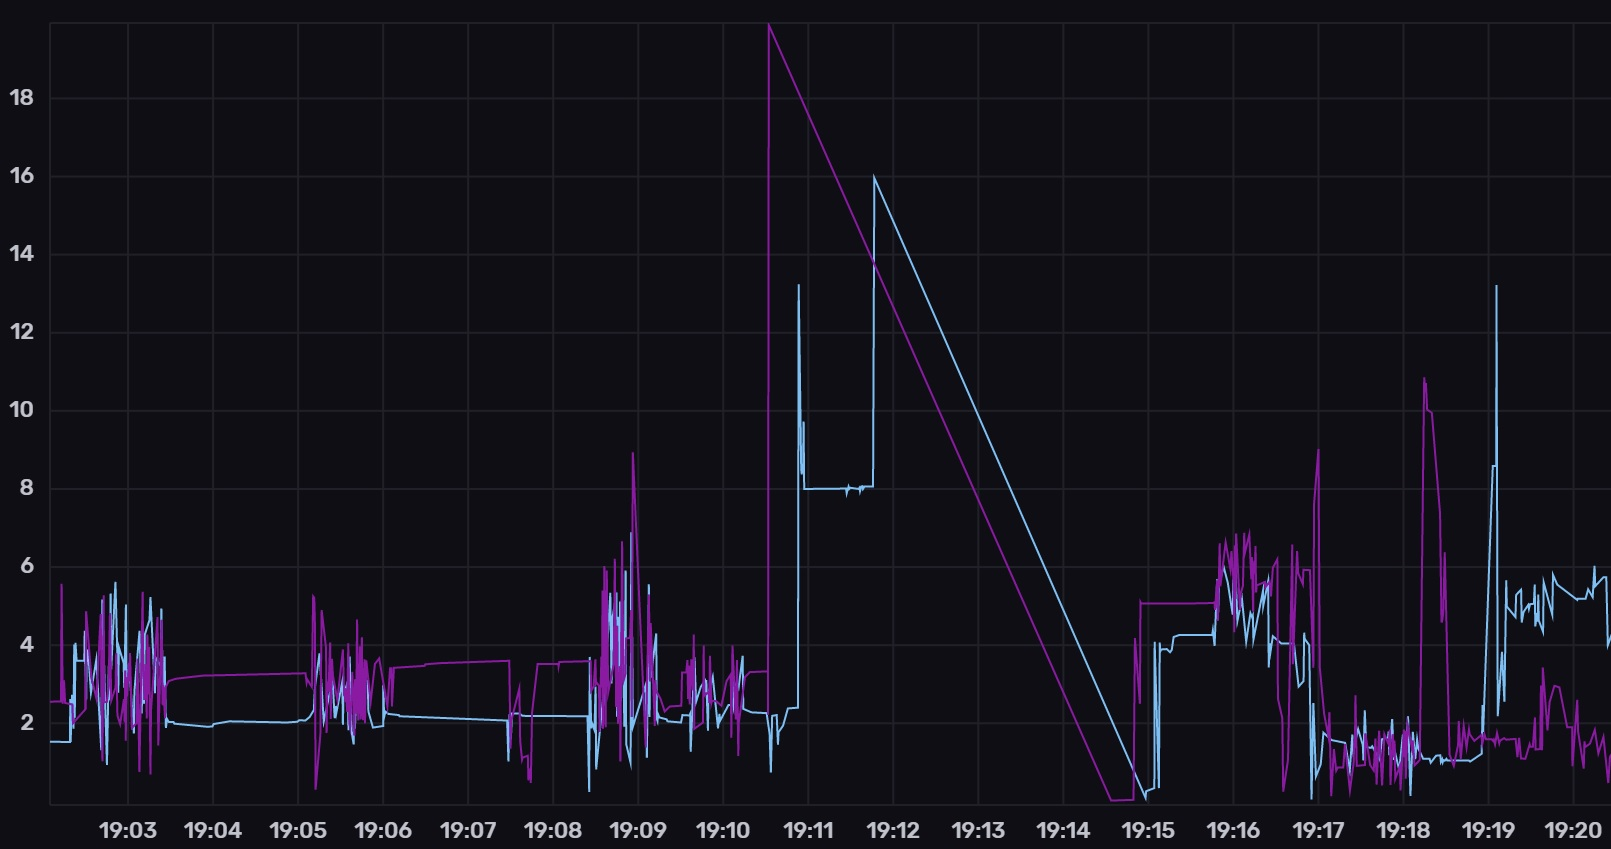
\includegraphics[width=\linewidth]{acc_2102}
	\caption{21 febbraio 2022, prima implementazione}
	\label{fig:accelerazione 2102}
\end{figure}

Con riferimento alla Figura 17, analizziamo questa lettura della prima implementazione.\\
Sull'asse delle ascisse è rappresentato il tempo, mentre sulle ordinate abbiamo l'accelerazione in $ m/s^2 $.
Il grafico può essere diviso in due parti da quel picco attorno alle 19 e 11, registrato da entrambi gli accelerometri,
seguito dalla loro momentanea disconnessione, fino alle 19 e 15. Le curve successive, e vedremo che questo sarà un 
problema ricorrente che tratteremo nelle conclusioni, presentano un andamento caotico e di difficile interpretazione.\\
La prima parte del grafico tuttavia mostra chiaramente tre serie di allenamento (zone "disturbate" del grafico), 
intervallate dai detti 90 secondi di pausa in cui entrambe le accelerazioni destra e sinistra rimangono costanti.
Da un lato è positivo il fatto che gli accelerometri scrivano correttamente le proprie letture, ma i dati relativi alla 
singola esecuzione, così come della serie intera, non offrono un andamento tale da trarre conclusioni o analisi.

Passiamo dunque al grafico della seconda implementazione, che segue in Figura 18.

\begin{figure}[htb]\centering
	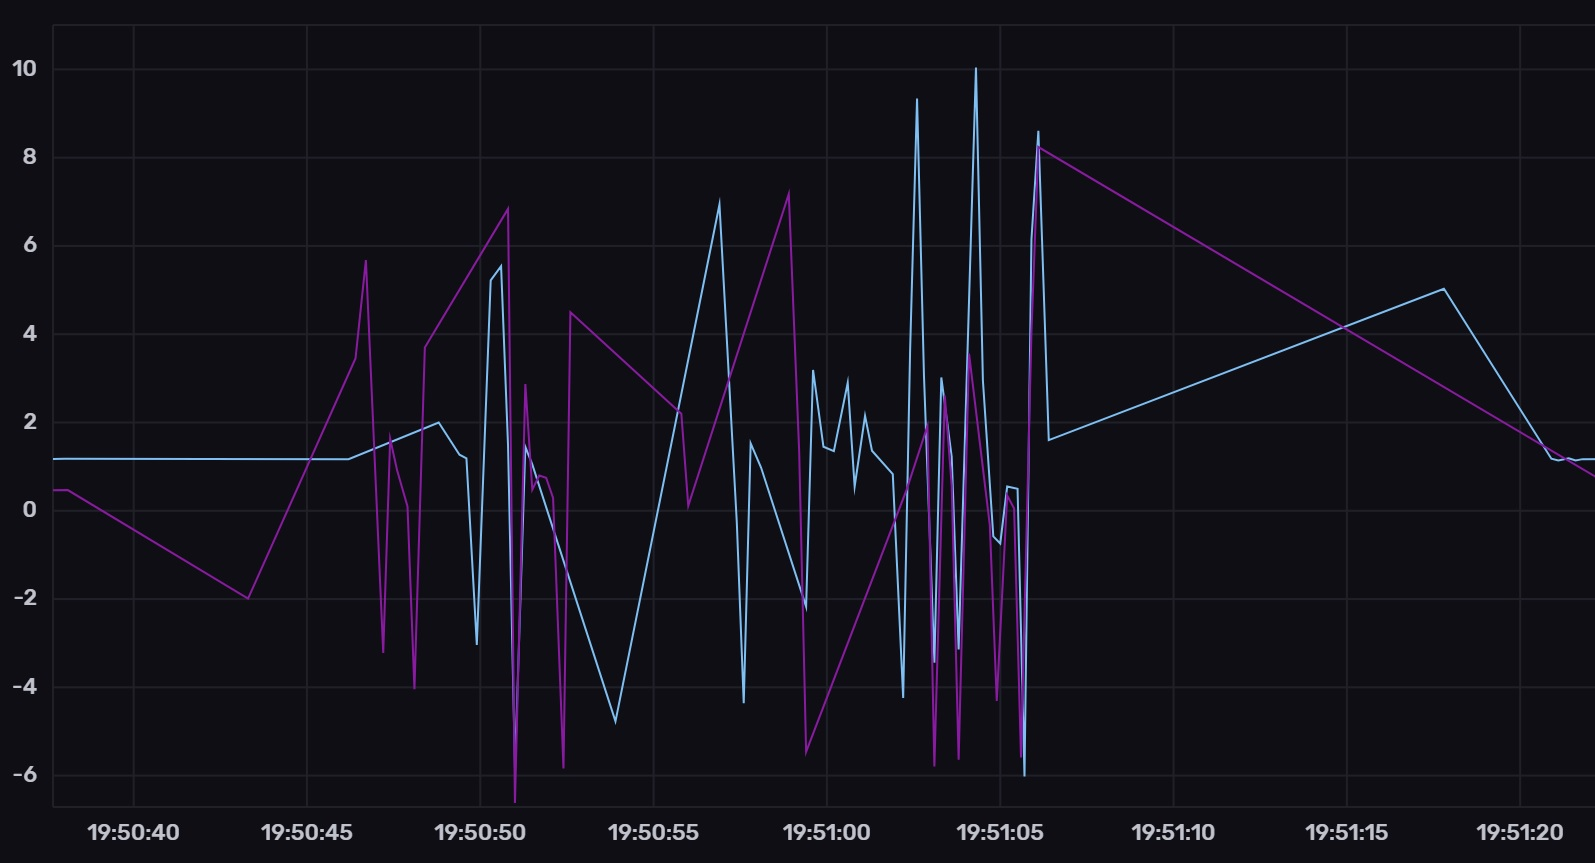
\includegraphics[width=\linewidth]{acc_0303}
	\caption{3 marzo 2022, seconda implementazione}
	\label{fig:accelerazione 0303}
\end{figure}

In questa fase erano stati fatti due importanti aggiornamenti al codice: in prima istanza era stata rimossa la tara alle 
misurazioni lungo gli assi cartesiani, in quanto ogni rotazione lungo l'asse orizzontale del bilanciere la rendeva del tutto 
inutile. Veniva comunque mantenuta la sottrazione dell'accelerazione di gravità dal vettore risultante. Inoltre era stata 
aumentata la granularità dei dati inviati, accorpando le misurazioni in array di 25 elementi, corrispondenti ad un invio 
di dati nominale ogni quarto di secondo (ricordando che 25 elementi corrispondono a 250 millesimi di secondo).\\
Il grafico, che questa volta riporta una sola serie dell'esercizio, mostra sicuramente un andamento più chiaro e coerente 
rispetto a quanto ricercato, in particolare le ultime tre ripetizioni sono ben rappresentate da aumenti e diminuzioni di 
accelerazione abbastanza allineati tra i due sensori.\\
Si può inoltre notare che l'accelerazione media in fase di discesa non raggiunge mai 1 g, a testimonianza di una discesa 
a velocità controllata del carico, contro una risalita abbastanza veloce, la cui accelerazione raggiunge i 10 $ m/s^2 $.\\

Nonostante l'evidente miglioramento, il risultato non è stato ritenuto soddisfacente anche alla luce dell'analisi dei dati 
tabellati (consultabili nel file allegato ACC\_ELAB\_2022-03-03.csv), che continuano a mostrare un evidente scostamento tra 
i valori dei due accelerometri, anche in presenza di un movimento costante e controllato del bilanciere.
Oltre a questo disturbo nelle misurazioni, risultava nuovamente evidente il progressivo degradarsi delle letture col passare 
dei minuti.\\

Con il successivo aggiornamento del codice è stata nuovamente modificata la dimensione dell'array, portandola a 30, diluendo 
in minima parte la frequenza di invio, con l'obiettivo di diminuire la perdita di dati inviati, che a questo punto iniziavamo 
a riconoscere come potenziale causa dello scostamento tra i dati registrati dai due accelerometri. Abbiamo inoltre raffinato 
il calcolo della media, effettuandolo non più sulle singole componenti prima di ricavare il vettore risultante, ma calcolando 
per ogni misurazione il vettore-somma, e successivamente la media tra tutti i vettori risultanti così ottenuti. Si è inoltre 
ritenuta superflua la normalizzazione attorno allo zero dell'accelerazione, che è stata rimossa.

\begin{figure}[htb]\centering
	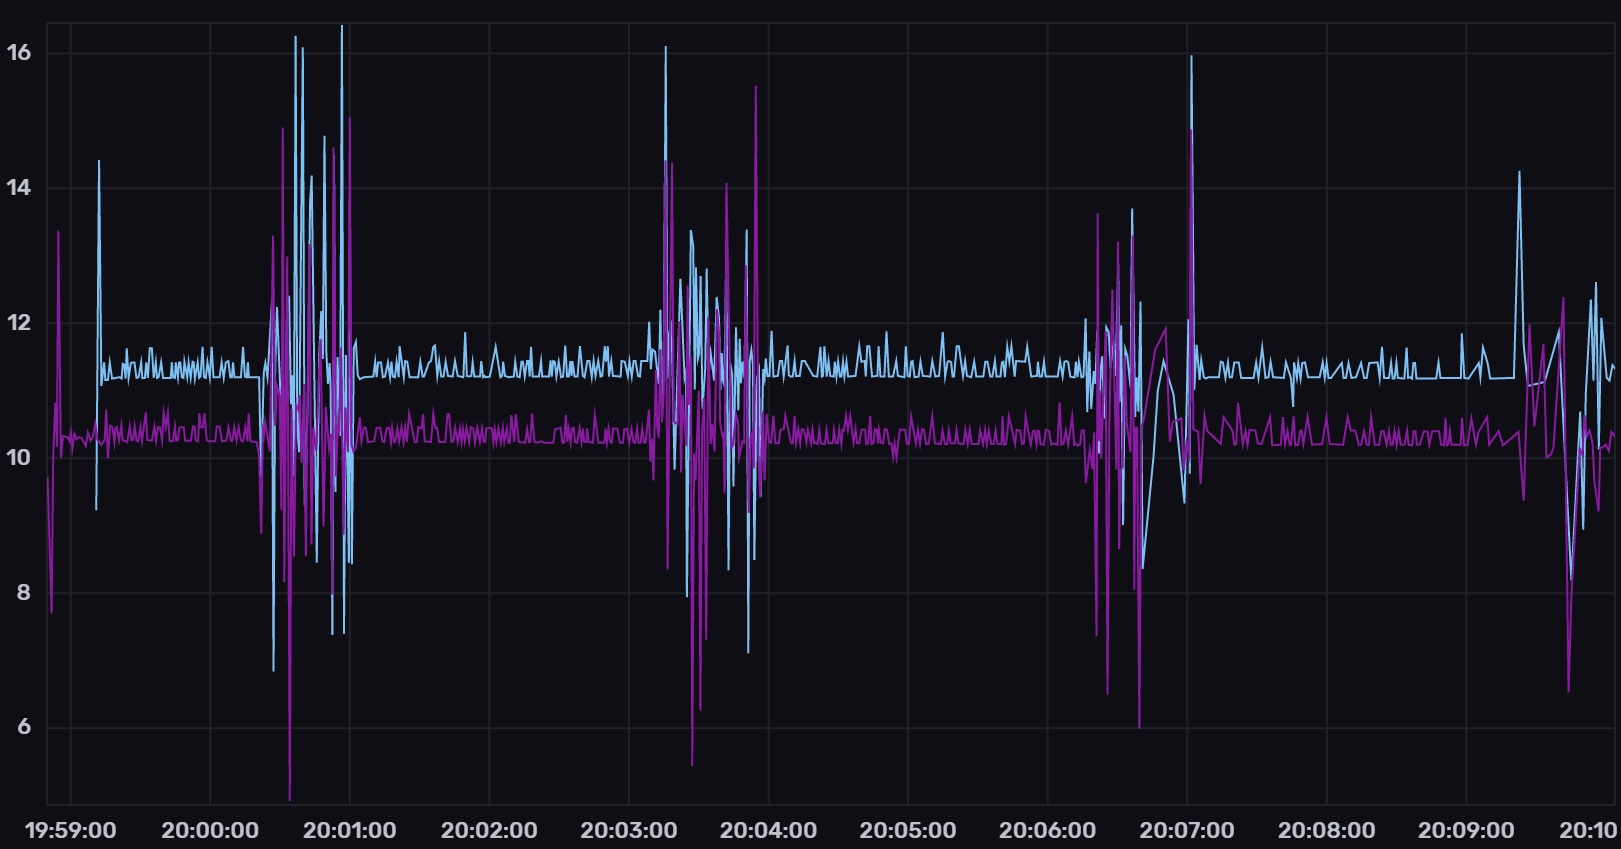
\includegraphics[width=\linewidth]{acc_2104}
	\caption{21 aprile 2022, terza implementazione}
	\label{fig:accelerazione 2104}
\end{figure}

\begin{figure}[htb]\centering
	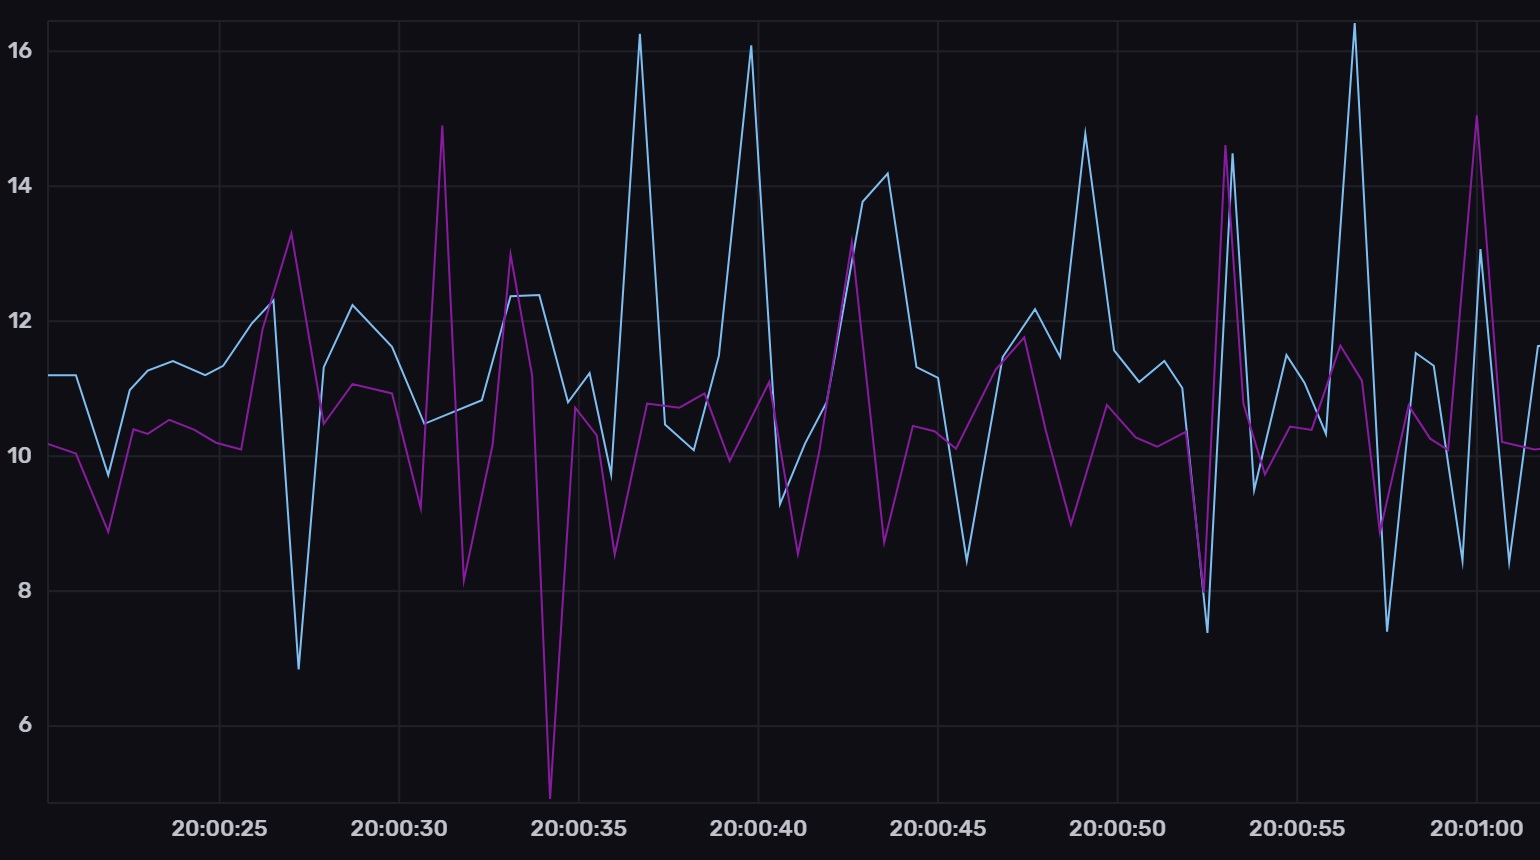
\includegraphics[width=\linewidth]{acc_2104_zoom}
	\caption{zoom sulla prima serie}
	\label{fig:zoom accelerazione 2104}
\end{figure}

In Figura 19 vediamo come gli aggiornamenti apportati abbiano reso i grafici molto più "armonici" rispetto alla prima versione 
del codice, pur mantenendo l'evidente degradarsi delle letture con il tempo.
Tuttavia lo zoom sulla singola serie (Figura 20) evidenzia come ancora una volta i dati ottenuti non siano coerenti con 
l'esecuzione controllata dell'esercizio, dalla quale ci si aspetterebbero due curve circa sovrapponibili, o al più lievemente 
discostate lungo l'asse del tempo.

\subsubsection{L'ultima versione del codice degli accelerometri}

Come nella precedente versione abbiamo di nuovo aumentato la dimensione dell'array a 35, con lo stesso obiettivo 
sopra descritto. In questa implementazione sono state tuttavia introdotte due ulteriori modifiche sostanziali:

\begin{itemize}[noitemsep] % [noitemsep] removes whitespace between the items for a compact look
	\item si è scelto di introdurre un'ulteriore metrica oltre alla media delle accelerazioni, ovvero il valore massimo di 
	ogni array. Questo semplicemente alla ricerca di nuovi dati che potessero meglio offrirsi a interpretazione.\\
	Possiamo anticipare che già dopo i primi test era stata riscontrata un'anomalia sulle letture dei sensori, che sporadicamente 
	registravano dei valori di accelerazione massima non plausibili (in modulo fino a 80 $ m/s^2 $), anomalia che ci ha mostrato 
	un probabile malfunzionamento dei sensori, aggirato con l'inserimento a livello di codice di valori soglia delle misurazioni, 
	oltre i quali il dato viene scartato. Trattandosi comunque di un'eventualità non troppo frequente, ciò non presenta 
	ripercussioni significative sulla sincronia delle letture dei due sensori.
	\item abbiamo deciso di parallelizzare i task principali dei moduli, sfruttando l'architettura dual core delle ESP32. 
	Invece di lavorare con il classico \textit{while-loop}, in fase di setup del microcontrollore vengono associati due task ai due 
	core, eseguiti a loro volta su \textit{cicli-for} infiniti. \\
	Uno dei due processori si occupa di raccogliere i dati, scrivendoli su un buffer 
	condiviso, l'altro controlla, come da paradigma produttore-consumatore, se ci sono dati pronti per essere elaborati (calcolo 
	della media e del massimo), e li invia. Il primo core, una volta riempito il primo array, passa a scrivere i dati su un 
	secondo buffer.\\
	L'idea di fondo è quella di permettere ad un core di effettuare continuamente le misurazioni, mentre all'altro di provvedere 
	ai calcoli sui dati e al successivo invio. Così facendo, ipotizzando l'assenza di problemi di perdita dati in fase di 
	comunicazione col server, si va ad annullare il tempo morto al termine del riempimento dell'array,
	consentendo una scrittura omogenea e continua sul database.
\end{itemize}

Possiamo osservare nelle immagini che seguono i grafici risultanti (Figure 21 e 22), di nuovo relativi ad una sola serie. 

\begin{figure}[htb]\centering
	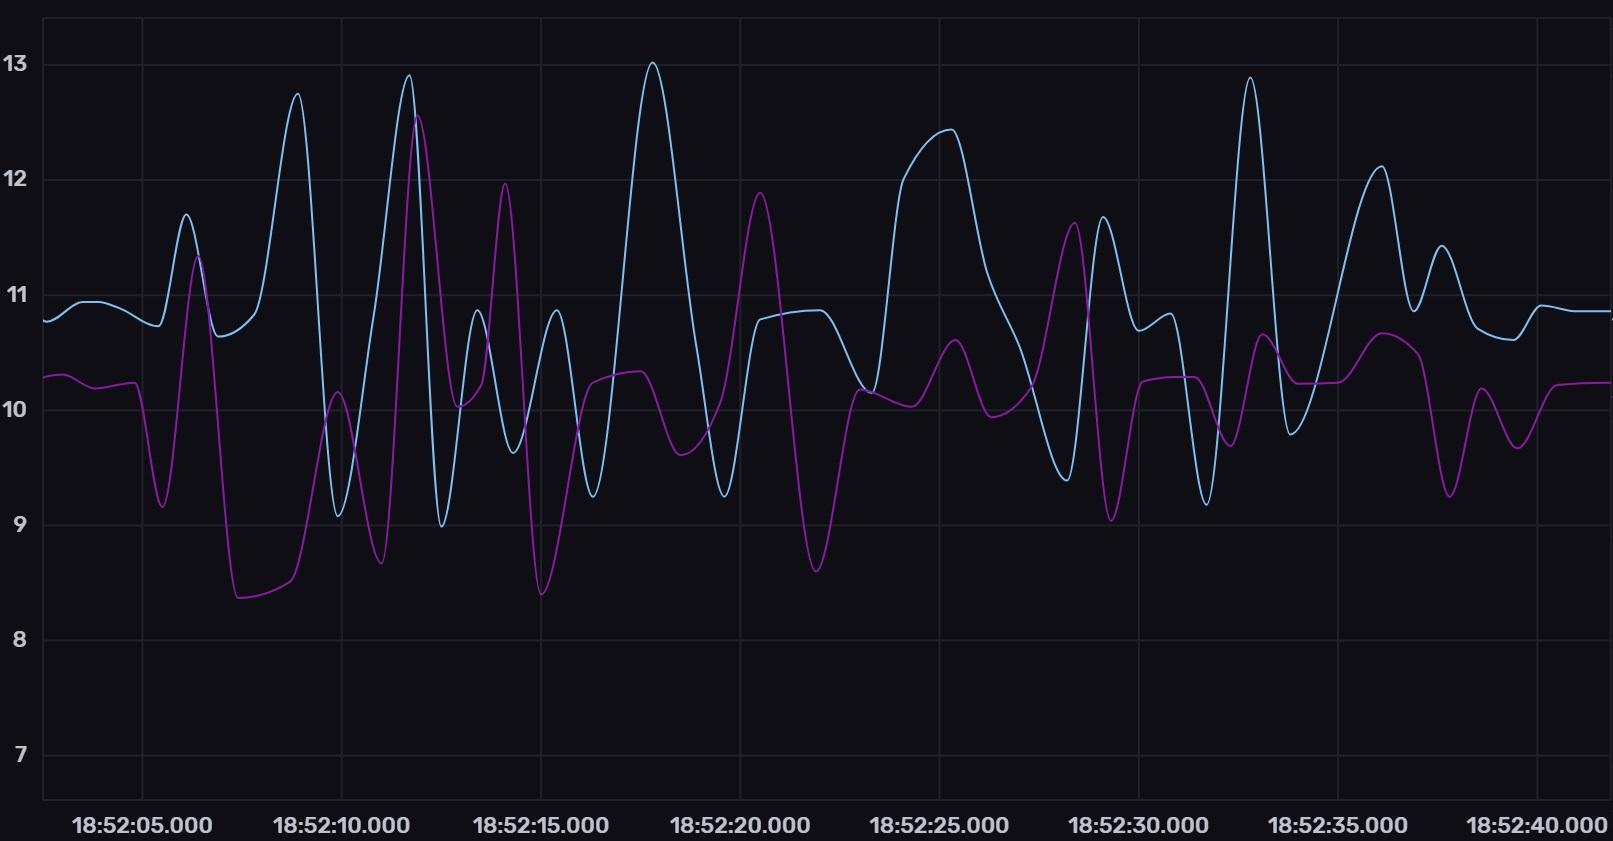
\includegraphics[width=\linewidth]{acc_0905_media}
	\caption{zoom sulla prima serie}
	\label{fig:zoom accelerazione 2104}
\end{figure}
\begin{figure}[htb]\centering
	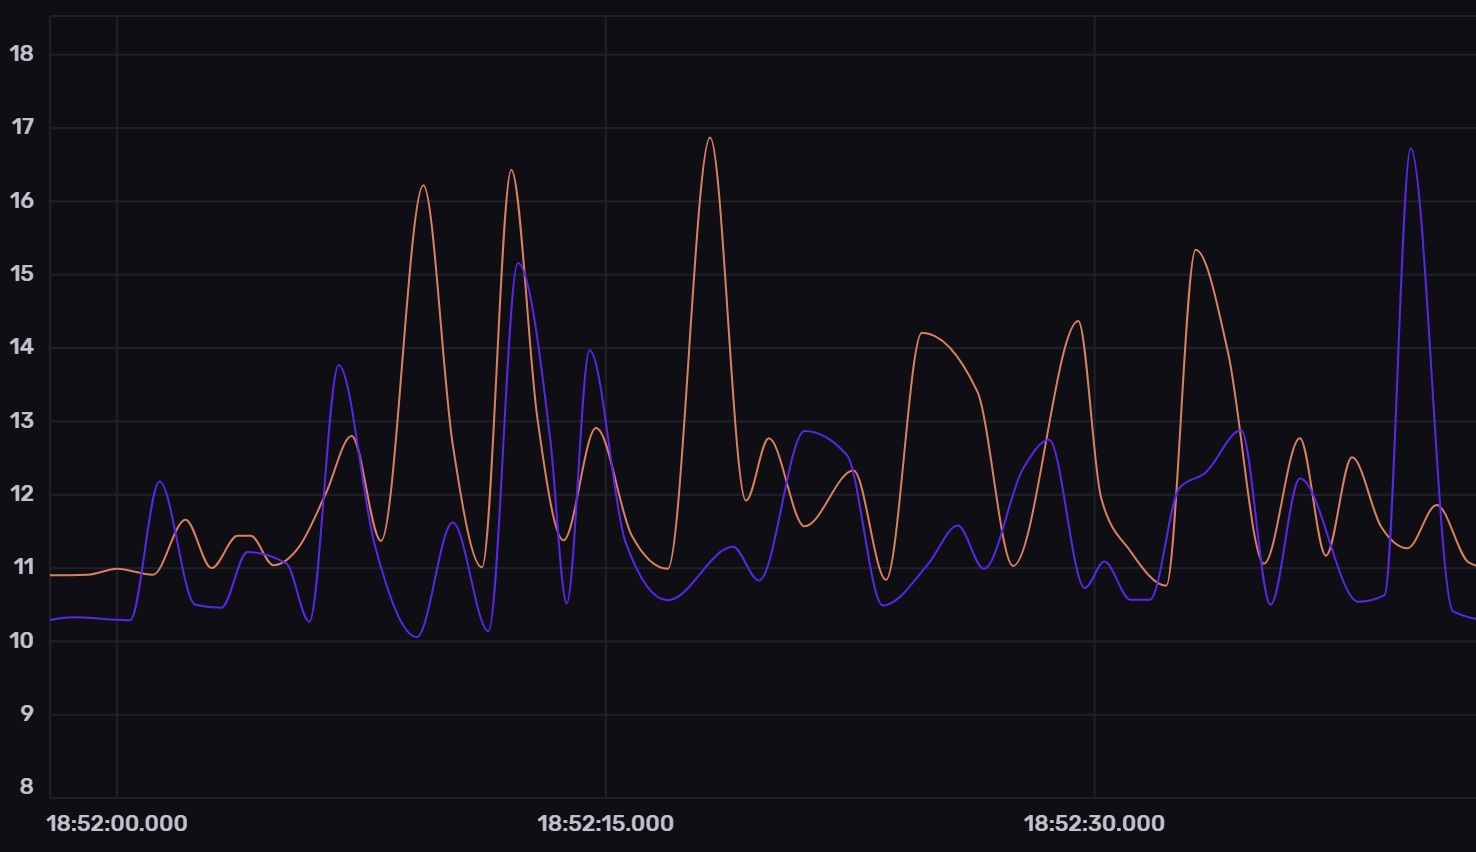
\includegraphics[width=\linewidth]{acc_0905_max}
	\caption{zoom sulla prima serie}
	\label{fig:zoom accelerazione 2104}
\end{figure}

Purtroppo ancora una volta, nonostante l'ulteriore accorgimento nell'utilizzo di un'interpolazione morbida nella generazione delle 
curve (selezionabile nelle impostazioni dei grafici di influxdb), ci troviamo di fronte a dati di difficile interpretazione, se non 
addirittura privi di significato.

\section{Analisi finale e conclusione}

\subsection{Risultati delle letture di temperatura e umidità}





\begin{figure}[htb]\centering
	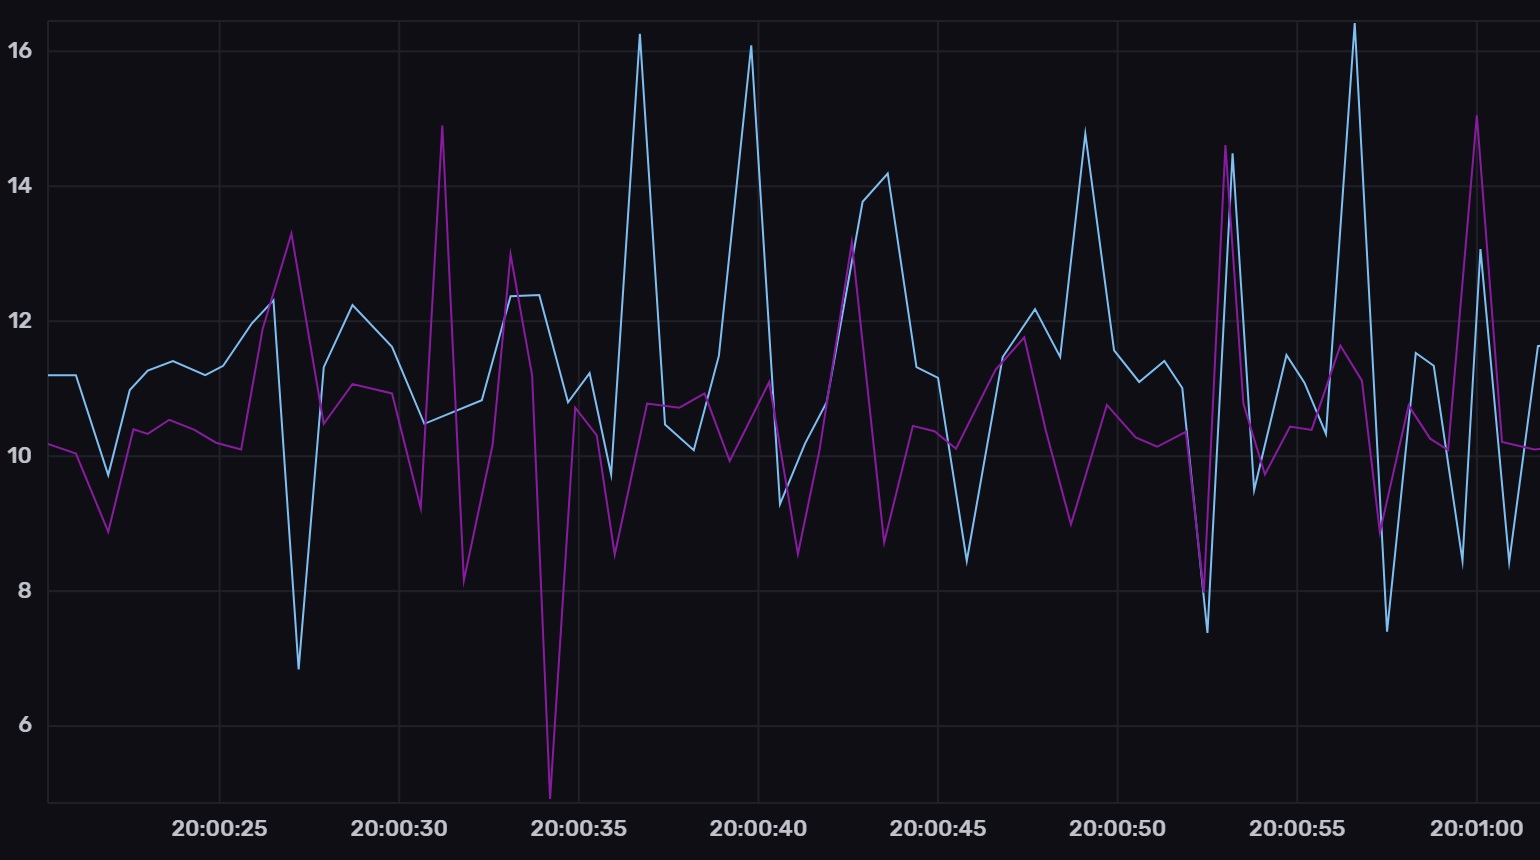
\includegraphics[width=\linewidth]{acc_2104_zoom}
	\caption{zoom sulla prima serie}
	\label{fig:zoom accelerazione 2104}
\end{figure}





\subsubsection{Subsubsection}

\section{Conclusioni}

%----------------------------------------------------------------------------------------
%	REFERENCE LIST
%----------------------------------------------------------------------------------------

\phantomsection
\bibliographystyle{unsrt}
\bibliography{sample.bib}

%----------------------------------------------------------------------------------------

\end{document}